\documentclass[a4paper,12pt,twoside]{memoir}

% Castellano
\usepackage[spanish,es-tabla]{babel}
\selectlanguage{spanish}
\usepackage[utf8]{inputenc}
\usepackage[T1]{fontenc}
\usepackage{lmodern} % scalable font
\usepackage{microtype}
\usepackage{placeins}

\usepackage{minted}
\usepackage{algpseudocode}

\usepackage{dirtree}


\usepackage{listings}             % Include the listings-package

\RequirePackage{booktabs}
\RequirePackage[table]{xcolor}
\RequirePackage{xtab}
\RequirePackage{multirow}
% Links
\PassOptionsToPackage{hyphens}{url}\usepackage[colorlinks]{hyperref}
\hypersetup{
	allcolors = {red}
}

% Ecuaciones
\usepackage{amsmath}

% Rutas de fichero / paquete
\newcommand{\ruta}[1]{{\sffamily #1}}

% Párrafos
\nonzeroparskip

% Huérfanas y viudas
\widowpenalty100000
\clubpenalty100000

% Evitar solapes en el header
\nouppercaseheads

% Imagenes
\usepackage{graphicx}
\newcommand{\imagen}[2]{
	\begin{figure}[!h]
		\centering
		\includegraphics[width=0.9\textwidth]{#1}
		\caption{#2}\label{fig:#1}
	\end{figure}
	\FloatBarrier
}

\newcommand{\imagenflotante}[2]{
	\begin{figure}%[!h]
		\centering
		\includegraphics[width=0.9\textwidth]{#1}
		\caption{#2}\label{fig:#1}
	\end{figure}
}



% El comando \figura nos permite insertar figuras comodamente, y utilizando
% siempre el mismo formato. Los parametros son:
% 1 -> Porcentaje del ancho de página que ocupará la figura (de 0 a 1)
% 2 --> Fichero de la imagen
% 3 --> Texto a pie de imagen
% 4 --> Etiqueta (label) para referencias
% 5 --> Opciones que queramos pasarle al \includegraphics
% 6 --> Opciones de posicionamiento a pasarle a \begin{figure}
\newcommand{\figuraConPosicion}[6]{%
  \setlength{\anchoFloat}{#1\textwidth}%
  \addtolength{\anchoFloat}{-4\fboxsep}%
  \setlength{\anchoFigura}{\anchoFloat}%
  \begin{figure}[#6]
    \begin{center}%
      \Ovalbox{%
        \begin{minipage}{\anchoFloat}%
          \begin{center}%
            \includegraphics[width=\anchoFigura,#5]{#2}%
            \caption{#3}%
            \label{#4}%
          \end{center}%
        \end{minipage}
      }%
    \end{center}%
  \end{figure}%
}

%
% Comando para incluir imágenes en formato apaisado (sin marco).
\newcommand{\figuraApaisadaSinMarco}[5]{%
  \begin{figure}%
    \begin{center}%
    \includegraphics[angle=90,height=#1\textheight,#5]{#2}%
    \caption{#3}%
    \label{#4}%
    \end{center}%
  \end{figure}%
}
% Para las tablas
\newcommand{\otoprule}{\midrule [\heavyrulewidth]}
%
% Nuevo comando para tablas pequeñas (menos de una página).
\newcommand{\tablaSmall}[5]{%
 \begin{table}
  \begin{center}
   \rowcolors {2}{gray!35}{}
   \begin{tabular}{#2}
    \toprule
    #4
    \otoprule
    #5
    \bottomrule
   \end{tabular}
   \caption{#1}
   \label{tabla:#3}
  \end{center}
 \end{table}
}

%
%Para el float H de tablaSmallSinColores
\usepackage{float}

%
% Nuevo comando para tablas pequeñas (menos de una página).
\newcommand{\tablaSmallSinColores}[5]{%
 \begin{table}[H]
  \begin{center}
   \begin{tabular}{#2}
    \toprule
    #4
    \otoprule
    #5
    \bottomrule
   \end{tabular}
   \caption{#1}
   \label{tabla:#3}
  \end{center}
 \end{table}
}

\newcommand{\tablaApaisadaSmall}[5]{%
\begin{landscape}
  \begin{table}
   \begin{center}
    \rowcolors {2}{gray!35}{}
    \begin{tabular}{#2}
     \toprule
     #4
     \otoprule
     #5
     \bottomrule
    \end{tabular}
    \caption{#1}
    \label{tabla:#3}
   \end{center}
  \end{table}
\end{landscape}
}

%
% Nuevo comando para tablas grandes con cabecera y filas alternas coloreadas en gris.
\newcommand{\tabla}[6]{%
  \begin{center}
    \tablefirsthead{
      \toprule
      #5
      \otoprule
    }
    \tablehead{
      \multicolumn{#3}{l}{\small\sl continúa desde la página anterior}\\
      \toprule
      #5
      \otoprule
    }
    \tabletail{
      \hline
      \multicolumn{#3}{r}{\small\sl continúa en la página siguiente}\\
    }
    \tablelasttail{
      \hline
    }
    \bottomcaption{#1}
    \rowcolors {2}{gray!35}{}
    \begin{xtabular}{#2}
      #6
      \bottomrule
    \end{xtabular}
    \label{tabla:#4}
  \end{center}
}

%
% Nuevo comando para tablas grandes con cabecera.
\newcommand{\tablaSinColores}[6]{%
  \begin{center}
    \tablefirsthead{
      \toprule
      #5
      \otoprule
    }
    \tablehead{
      \multicolumn{#3}{l}{\small\sl continúa desde la página anterior}\\
      \toprule
      #5
      \otoprule
    }
    \tabletail{
      \hline
      \multicolumn{#3}{r}{\small\sl continúa en la página siguiente}\\
    }
    \tablelasttail{
      \hline
    }
    \bottomcaption{#1}
    \begin{xtabular}{#2}
      #6
      \bottomrule
    \end{xtabular}
    \label{tabla:#4}
  \end{center}
}

%
% Nuevo comando para tablas grandes sin cabecera.
\newcommand{\tablaSinCabecera}[5]{%
  \begin{center}
    \tablefirsthead{
      \toprule
    }
    \tablehead{
      \multicolumn{#3}{l}{\small\sl continúa desde la página anterior}\\
      \hline
    }
    \tabletail{
      \hline
      \multicolumn{#3}{r}{\small\sl continúa en la página siguiente}\\
    }
    \tablelasttail{
      \hline
    }
    \bottomcaption{#1}
  \begin{xtabular}{#2}
    #5
   \bottomrule
  \end{xtabular}
  \label{tabla:#4}
  \end{center}
}



\definecolor{cgoLight}{HTML}{EEEEEE}
\definecolor{cgoExtralight}{HTML}{FFFFFF}

%
% Nuevo comando para tablas grandes sin cabecera.
\newcommand{\tablaSinCabeceraConBandas}[5]{%
  \begin{center}
    \tablefirsthead{
      \toprule
    }
    \tablehead{
      \multicolumn{#3}{l}{\small\sl continúa desde la página anterior}\\
      \hline
    }
    \tabletail{
      \hline
      \multicolumn{#3}{r}{\small\sl continúa en la página siguiente}\\
    }
    \tablelasttail{
      \hline
    }
    \bottomcaption{#1}
    \rowcolors[]{1}{cgoExtralight}{cgoLight}

  \begin{xtabular}{#2}
    #5
   \bottomrule
  \end{xtabular}
  \label{tabla:#4}
  \end{center}
}




\graphicspath{ {./img/} }

% Capítulos
\chapterstyle{bianchi}
\newcommand{\capitulo}[2]{
	\setcounter{chapter}{#1}
	\setcounter{section}{0}
	\chapter*{#2}
	\addcontentsline{toc}{chapter}{#2}
	\markboth{#2}{#2}
}

% Apéndices
\renewcommand{\appendixname}{Apéndice}
\renewcommand*\cftappendixname{\appendixname}

\newcommand{\apendice}[1]{
	%\renewcommand{\thechapter}{A}
	\chapter{#1}
}

\renewcommand*\cftappendixname{\appendixname\ }

% Formato de portada
\makeatletter
\usepackage{xcolor}
\newcommand{\tutor}[1]{\def\@tutor{#1}}
\newcommand{\course}[1]{\def\@course{#1}}
\definecolor{cpardoBox}{HTML}{E6E6FF}
\def\maketitle{
  \null
  \thispagestyle{empty}
  % Cabecera ----------------
\noindent
\includegraphics[width=\textwidth]{cabecera}\vspace{1cm}%
  \vfill
  % Título proyecto y escudo informática ----------------
  \colorbox{cpardoBox}{%
    \begin{minipage}{.8\textwidth}
      \vspace{.5cm}\Large
      \begin{center}
      \textbf{TFG del Grado en Ingeniería Informática}\vspace{.6cm}\\
      \textbf{\LARGE\@title{}}
      \end{center}
      \vspace{.2cm}
    \end{minipage}

  }%
  \hfill\begin{minipage}{.20\textwidth}
    
\includegraphics[width=\textwidth]{escudoInfor}
  \end{minipage}
  \vfill
  % Datos de alumno, curso y tutores ------------------
  \begin{center}%
  {%
    \noindent\LARGE
    Presentado por \@author{}\\ 
    en Universidad de Burgos --- \@date{}\\
    Tutor: \@tutor{}\\
  }%
  \end{center}%
  \null
  \cleardoublepage
  }
\makeatother


% Datos de portada
\title{Monitorización sensores IOT}
\author{Daniel Mellado Hurtado}
\tutor{Bruno Baruque Zanon}
\date{\today}

\newcommand{\nombrePrograma}{Monitorizacion\_IOT } %%% cambio de comando

\begin{document}

\maketitle



\cleardoublepage



%%%%%%%%%%%%%%%%%%%%%%%%%%%%%%%%%%%%%%%%%%%%%%%%%%%%%%%%%%%%%%%%%%%%%%%%%%%%%%%%%%%%%%%%



\frontmatter


\clearpage

% Indices
\tableofcontents

\clearpage

\listoffigures

\clearpage

\listoftables

\clearpage

\mainmatter

\appendix

\apendice{Plan de Proyecto Software}

\section{Introducción}

La planificación y el seguimiento de metodologías de desarrollo es esencial para el éxito de cualquier proyecto. En esta sección se describirá la planificación temporal que se ha seguido del proyecto, así como el estudio de viabilidad del mismo.

\section{Planificación temporal}

Para la realización del proyecto se ha optado por la utilización del método \textbf{Scrum}, una metodología ágil de gestión de proyectos en la  que se ha dividido el desarrollo en \textbf{sprints} de aproximadamente 2 semanas de duración en la que había una reunión con el tutor y se planteaban las próximas tareas que se iban a realizar.

Para la organización de tareas se utilizó una tabla con 6 columnas:

\begin{itemize}
    \item \textbf{Procut Backlog}: En esta columna se colocan las tareas que se han de realizar a lo largo del proyecto.
    \item \textbf{Sprint Backlog}: Al inicio de cada sprint se mueven a esta columna las tareas que se planea realizar durante el transcurso de dicho sprint.
    \item \textbf{In Progress}: En esta columna se encuentran todas aquellas tareas que se están realizando en ese momento.
    \item \textbf{Review/QA}: Cuando en alguna tarea sea necesario realizar una revisión por parte del propio desarrollador cómo por parte del tutor se mueve a esta columna.
    \item \textbf{Done}: Cuando las tareas ya han sido finalizadas se mueven a esta columna
    \item \textbf{IceBox}: En esta última columna se colocan las tareas que han sido abandonadas o que tienen muy baja prioridad.
\end{itemize}


La planificación de las tareas se puede consultar en GitHub en el repositorio: \url{https://github.com/dmh1001/TFG-Monitorizacion-IOT}

Debido a la situación actual del COVID-19 las reuniones se llevaron a cabo mediante videollamadas por \textbf{Microsoft Teams}

\subsection{Sprint 0 - Introducción (30/11/2020 - 14/12/2020)}

Durante este \textbf{Sprint} lo principal fue investigar sobre las posibles herramientas que se podrían utilizar en este proyecto así cómo documentar dichas herramientas en la memoria.

Durante esta parte del proyecto se creó el repositorio de Github y se instaló ZenHub para gestionar las issues del proyecto.

\subsection{Sprint 1   (14/12/2020 - 04/01/2021 )}

Durante este \textbf{Sprint} se especificaron cuáles serían los objetivos del proyecto, se decidieron las herramientas que se iban a utilizar y se comenzó con su documentación en la memoria.

\subsection{Sprint 2   (04/01/2021 - 06/02/2021 )}

Durante este \textbf{Sprint} se instaló el servidor PRTG en una máquina virtual Windows 10 así cómo Elasticsearch. 

\subsection{Sprint 3   (06/02/2021 - 25/02/2021 )}

Durante este \textbf{Sprint} se instaló Elasticsearch, programa el cual serviría de BBDD y monitorización de nuestros sensores, en un equipo con sistema Window y se procedió a conectarlo con PRTG. 

\subsection{Sprint 4   (25/02/2021 - 12/03/2021 )}
Durante este \textbf{Sprint} se migro Elasticsearch a una máquina Virtual Ubuntu server para poder simular un servidor real.


\subsection{Sprint 5   (12/03/2021 - 26/03/2021 )}

Durante este \textbf{Sprint} se fue estructurando y creando el manual de instalación con lo desarrollado hasta la fecha.

\subsection{Sprint 6 - Conectividad PRTG-ELK (28/03/2021 - 12/04/2021 )}
En este \textbf{Sprint} se finaliza con la conexión entre PRTG y Elasticsearch, Se idea una forma de transformar los datos procedentes de PRTG mediante un sencillo programa en Flex para que los datos sean más fáciles de leer por logstash.

Con los datos obtenidos y almacenados el Elasticsearch se pudo empezar a monitorizar los datos gracias a Kibana

\subsection{Sprint 7 - acercamiento machine learning  (12/04/2021 - 26/04/2021 )}
En este \textbf{Sprint} se investigó las diferentes librerías y técnicas  
de machine learning y predicción de datos.

\subsection{Sprint 8 (1/05/2021 - 10/05/2021 )}
En este \textbf{Sprint} se configuró los sensores de la bodega y se desarrolló una función que permitía descargar los datos de Elasticsearch al servidor.

Además, se realizaron diversas pruebas y tutórales con algoritmos de machine learning para aprender y decidir cuáles serían los más apropiados en el proyecto.

\subsection{Sprint 9   (15/05/2021 - 10/06/2021 )}

En este \textbf{Sprint} se creó el modelo y se desarrolló una función capaz de devolver los datos predichos por el modelo a Elasticsearch para poder ser visualizados.

\subsection{Sprint 10  (10/06/2021 - 24/06/2021 )}
En este \textbf{Sprint} se realizaron una seré de funciones que permitían guardar y cargar el modelo al programa.

También se refactorizó el código para aumentar su legibilidad y mantener un formato y una coherencia.

\subsection{Sprint 11  (31/08/2021 - 14/09/2021 )}
En este \textbf{Sprint} se implementaron nuevos modelos y se facilitó la creación de otros en el futuro.

Se detecto un error a la hora de descargar los datos de PRTG y transformar los datos y se decidió migrar la funcionalidad de transformación de datos de Flex a Python.

Se fue redactando la memoria para dejarla finalizada para la entrega.


\begin{figure}[h]
	\centering
	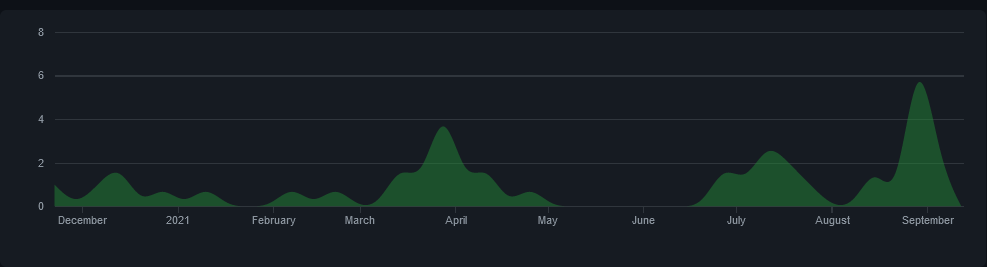
\includegraphics[width=1.1\textwidth]{img/img_grafico_github.png}
	\caption{Gráfico de commits realizados en el tiempo}
	\label{img_grafico_github}
\end{figure}
\newpage

\section{Estudio de viabilidad}

Antes de adentrarse en la realización de cualquier proyecto se ha de estudiar su viabilidad en el mercado, estimar que costes se van a tener y que beneficios se van a obtener. Durante este apartado se verá la viabilidad tanto económica como legar del proyecto.

\subsection{Viabilidad económica}
A continuación, se hará un estudio sobre los costes y beneficios del proyecto si este se hubiera realizado en un ambiente empresarial real.

\subsubsection{Costes}

\subsubsubsection{\textbf{Costes personales}}

El desarrollo del proyecto ha sido realizado por un desarrollador junior, suponiendo que el salario bruto mensual es de 2000€.

\tablaSmallSinColores{Costes de personal}{p{6.4cm} p{2.15cm} p{8cm}}{costes personales}{
  \multicolumn{1}{p{4.5cm}}{\textbf{Concepto}} & \textbf{Coste{}}\\
 }{
Salario mensual neto  & \multicolumn{1}{r}{1217.25}\\
Retención IRPF (15\%) & \multicolumn{1}{r}{216.75}\\
Seguridad social  (28.3\%) & \multicolumn{1}{r}{566}\\
Salario mensual bruto  & \multicolumn{1}{r}{2000}\\\hline
\textbf{Coste total (6 meses)}  & \multicolumn{1}{r}{12000}\\
}

\subsubsubsection{\textbf{Costes hardware}}

En este apartado se mostrará el coste de los dispositivos hardware empleados para el desarrollo del proyecto. Dado que este se ha realizado durante 8 meses y suponiendo que la amortización es de 4 años.
  
\tablaSmallSinColores{Coste hardware}{p{3.4cm} p{1.15cm} p{4cm}}{Coste hardware}{
  \multicolumn{1}{p{4.5cm}}{\textbf{Concepto}} & \textbf{Coste{}} & \textbf{Amortización{}}\\
 }{
  Ordenador  & \multicolumn{1}{r}{1200€} & \multicolumn{1}{r}{50€}\\
  }
  
\subsubsubsection{\textbf{Costes software}}

En este apartado se revisarán los costes asociados a licencias de software no gratuitos. Consideraremos que la amortización del software es de 2 años.

\tablaSmallSinColores{Coste Software}{p{3.4cm} p{1.15cm} p{4cm}}{Coste Software}{
  \multicolumn{1}{p{4.5cm}}{\textbf{Concepto}} & \textbf{Coste} & \textbf{Amortización}\\
 }
 {
  Windows 10 pro  & \multicolumn{1}{r}{259€} & \multicolumn{1}{r}{5.4€}\\
   \multicolumn{1}{r}{}\\
  }
  
\subsubsection{Beneficios}

Al tratarse de un proyecto estudiantil es muy complicado estimar un beneficio. 

\subsection{Viabilidad legal}

Para poder distribuir un producto software es necesario cumplir ciertas obligaciones legales como son el caso de las licencias.

A continuación, se mostrarán las licencias del software empleado.


\tablaSmallSinColores{Licencias}{p{4.4cm} p{6.15cm} p{4cm}}{licencias}{
  \multicolumn{1}{p{4.5cm}}{\textbf{Herramienta}} & \textbf{Licencia}\\
 }
 {
  Elasticsearch  & \multicolumn{1}{r}{}\\
  PRTG  & \multicolumn{1}{r}{}\\
  virtualBox  & \multicolumn{1}{r}{}\\
  Ubuntu  & \multicolumn{1}{r}{}\\
  Windows 10  & \multicolumn{1}{r}{}\\
  Git  & \multicolumn{1}{r}{GPL2}\\
  GitHub  & \multicolumn{1}{r}{Propietaria/Privativa}\\
   \multicolumn{1}{r}{}\\
  }

\apendice{Especificación de Requisitos}

\section{Introducción}

En este anexo se recogen los objetivos del proyecto y los requisitos que definen el comportamiento del programa.

\section{Objetivos generales}

Con este proyecto se persigue la realización de los siguientes objetivos:

\begin{itemize}
    \item La instalación y configuración de un sistema capaz de recoger, almacenar y gestionar datos de sensores.
    \item La implementación de un motor de búsqueda para facilitar encontrar los datos deseados con la mayor precisión posible.
    \item Que la monitorización de los datos se muestre lo más clara y accesible posible para el usuario.
    \item Realizar un algoritmo de aprendizaje automático que pueda predecir comportamientos y patrones en los datos de los sensores.
\end{itemize}

\newpage
\section{Catálogo de requisitos}
A continuación, se procederá a enumerar los distintos requisitos funcionales:


\begin{itemize}

    \item \textbf{RF-1 Activar sistema}: El usuario ha de poder activar el sistema cuando desee.
    
    \item \textbf{RF-2 Desactivar sistema}: El usuario ha de poder desactivar el sistema cuando desee.
    
    \item \textbf{RF-3 Captación de sensores}: El sistema ha de almacenar los datos procedentes de los sensores.
    	
    \item \textbf{RF-4 Entrenamiento}: El sistema ha de entrenar un modelo con los datos de los sensores.

    \item \textbf{RF-5 Predicción}: El sistema ha de realizar una predicción sobre los datos de los sensores.

    \item \textbf{RF-6 Gestión del sistema}: El usuario ha de ser capaz de gestionar el sistema.
    \begin{itemize}
	    \item \textbf{RF-6.1 Añadir sensor}: El usuario ha de poder añadir sensores.
	    \item \textbf{RF-6.2 Borrar sensor}: El usuario ha de poder eliminar sensores.
	    \item \textbf{RF-6.3 Configurar modelo}: El usuario ha de poder configurar sus propios modelos.
	\end{itemize}
	
	\item \textbf{RF-7 Monitorización de datos}: El usuario ha de poder ver los datos de los sensores.
	\begin{itemize}
	    \item \textbf{RF-7.1 ver datos reales}: Se ha de monitorizar los datos reales procedentes del sensor.
	    \item \textbf{RF-7.2 ver datos entrenamiento}: Se ha de monitorizar los datos de entrenamiento del modelo.
	    \item \textbf{RF-7.3 ver datos predicción}: Se ha de monitorizar los datos de predicción.
	\end{itemize}
	\item \textbf{RF-8 Búsquedas filtradas}: El usuario ha de ser capaz de hacer búsquedas y filtrados de los datos.
	\item \textbf{RF-9 Representación gráfica}: El usuario ha de poder representar de forma gráfica los datos.
	\begin{itemize}
	    \item \textbf{RF-9.1 Creación de gráficas}: El usuario ha de poder crear gráficas.
	    \item \textbf{RF-9.2 Borrado de gráficas}: El usuario ha de poder borrar gráficas.
	    \item \textbf{RF-9.3 Visualización de gráficas}: El usuario ha de poder visualizar y consultar las gráficas creadas.
	\end{itemize}
	
\end{itemize}	
\newpage



\section{Especificación de requisitos}

En esta sección se mostrarán los casos de uso y su diagrama.

\subsection{Diagrama de casos de uso}

\begin{figure}[!h]
	\centering
	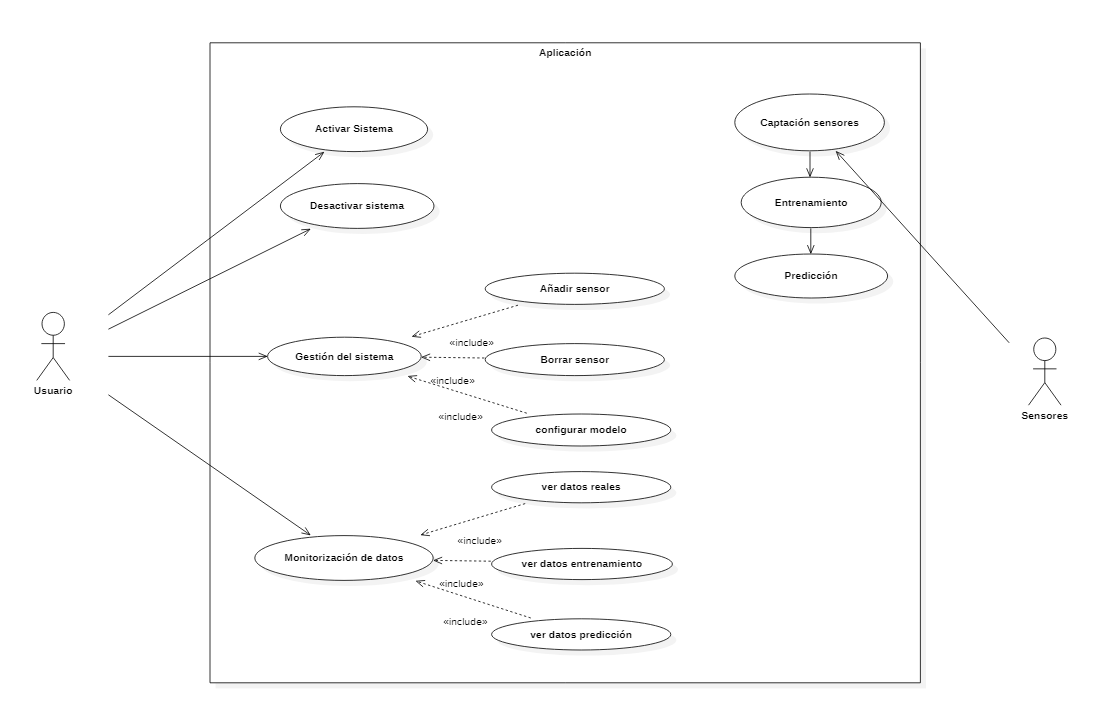
\includegraphics[width=1.2\textwidth]{img/img_casos_usos.png}
	\caption{Diagrama de casos de uso}
	\label{img_casos_usos}
\end{figure}
\clearpage

\subsection{Actores}
En esta aplicación interactúan dos actores, los sensores de los que se captan la información y el usuario que gestiona la aplicación y monitoriza el sistema.

\subsection{Casos de uso}
%Caso de uso 1
\tablaSmallSinColores{Caso de uso 1: Activar sistema.}{p{3cm} p{.75cm} p{9.5cm}}{tablaUC0}{
  \multicolumn{3}{l}{Caso de uso 1: Activar sistema.} \\
 }
 {
  Versión                            & \multicolumn{2}{p{10.25cm}}{1.0} \\\hline
  Autor                            & \multicolumn{2}{p{10.25cm}}{Daniel Mellado Hurtado} \\\hline
  Descripción                            & \multicolumn{2}{p{10.25cm}}{El usuario ha de poder activar el sistema cuando desee.} \\\hline
  \multirow{2}{3.5cm}{Requisitos}   &\multicolumn{2}{p{10.25cm}}{RF-1} \\\cline{2-3}

                                         \\\hline
                                         
  Precondiciones                         &  \multicolumn{2}{p{10.25cm}}{El programa ha de estar correctamente instalado.}   \\\hline
  \multirow{2}{3.5cm}{Secuencia normal}  & Paso & Acción \\\cline{2-3}
                                         & 1    & El usuario introduce el comando de inicialización del programa en la consola
  

                                         \\\hline
  Postcondiciones                        & \multicolumn{2}{p{10.25cm}}{El sistema se encuentra activo y funcionando} \\\hline
  Excepciones                        & \multicolumn{2}{p{10.25cm}}{No se encuentra el servicio correspondiente al programa.}\\\hline
  Importancia                            & Alta \\\hline
  Urgencia                               & Alta \\
}

%Caso de uso 2
\tablaSmallSinColores{Caso de uso 2: Desactivar sistema.}{p{3cm} p{.75cm} p{9.5cm}}{tablaUC0}{
  \multicolumn{3}{l}{Caso de uso 2: Desactivar sistema.} \\
 }
 {
  Versión                            & \multicolumn{2}{p{10.25cm}}{1.0} \\\hline
  Autor                            & \multicolumn{2}{p{10.25cm}}{Daniel Mellado Hurtado} \\\hline
  Descripción                            & \multicolumn{2}{p{10.25cm}}{El usuario ha de poder desactivar el sistema cuando desee.} \\\hline
  \multirow{2}{3.5cm}{Requisitos}   &\multicolumn{2}{p{10.25cm}}{RF-2} \\\cline{2-3}

                                         \\\hline
                                         
  Precondiciones                         &  \multicolumn{2}{p{10.25cm}}{El sistema se encuentra activo}   \\\hline
  \multirow{2}{3.5cm}{Secuencia normal}  & Paso & Acción \\\cline{2-3}
                                         & 1    & El usuario introduce el comando de parada del programa en la consola


                                         \\\hline
  Postcondiciones                        & \multicolumn{2}{p{10.25cm}}{El sistema se encuentra desactivado} \\\hline
  Excepciones                        & \multicolumn{2}{p{10.25cm}}{}\\\hline
  Importancia                            & Alta \\\hline
  Urgencia                               & Alta \\
}

%Caso de uso 3
\tablaSmallSinColores{Caso de uso 3: Almacenamiento de datos.}{p{3cm} p{.75cm} p{9.5cm}}{tablaUC0}{
  \multicolumn{3}{l}{Caso de uso 3: Almacenamiento de datos.} \\
 }
 {
  Versión                            & \multicolumn{2}{p{10.25cm}}{1.0} \\\hline
  Autor                            & \multicolumn{2}{p{10.25cm}}{Daniel Mellado Hurtado} \\\hline
  Descripción                            & \multicolumn{2}{p{10.25cm}}{El sistema ha de almacenar los datos procedentes de los sensores} \\\hline
  \multirow{2}{3.5cm}{Requisitos}   &\multicolumn{2}{p{10.25cm}}{RF-3} \\\cline{2-3}

                                         \\\hline
                                         
  Precondiciones                         &  \multicolumn{2}{p{10.25cm}}{Los sensores se encuentran activos y PRTG recibe sus datos}   \\\hline
  \multirow{2}{3.5cm}{Secuencia normal}  & Paso & Acción \\\cline{2-3}
                                         & 1    & El sistema descarga los datos procedentes de PRTG
  \\\cline{2-3}
                                         & 2    & Se transforman los datos descargados
    \\\cline{2-3}
                                         & 3    & El sistema envía los datos a Elasicsearch 
                                         \\\hline
  Postcondiciones                        & \multicolumn{2}{p{10.25cm}}{Los datos de los sensores son recogidos y almacenados correctamente} \\\hline
  Excepciones                        & \multicolumn{2}{p{10.25cm}}{No se encuentra el servidor de PRTG. No hay datos disponibles}\\\hline
  Importancia                            & Alta \\\hline
  Urgencia                               & Alta \\
}

%Caso de uso 4
\tablaSmallSinColores{Caso de uso 4: Entrenamiento.}{p{3cm} p{.75cm} p{9.5cm}}{tablaUC0}{
  \multicolumn{3}{l}{Caso de uso 4: Entrenamiento.} \\
 }
 {
  Versión                            & \multicolumn{2}{p{10.25cm}}{1.0} \\\hline
  Autor                            & \multicolumn{2}{p{10.25cm}}{Daniel Mellado Hurtado} \\\hline
  Descripción                            & \multicolumn{2}{p{10.25cm}}{El sistema ha de entrenar un modelo con los datos de los sensores} \\\hline
  \multirow{2}{3.5cm}{Requisitos}   &\multicolumn{2}{p{10.25cm}}{RF-4} \\\cline{2-3}
                                         & \multicolumn{2}{p{10.25cm}}{}
                                         \\\hline
                                         
  Precondiciones                         &  \multicolumn{2}{p{10.25cm}}{Existen datos de los sensores en Elasitcsearch. Exista un modelo para cada sensor que se vaya a entrenar}   \\\hline
  \multirow{2}{3.5cm}{Secuencia normal}  & Paso & Acción \\\cline{2-3}
                                         & 1    & El sistema descarga los datos que se desea entrenar de Elasticsearch
  \\\cline{2-3}
                                         & 2    & Se carga el modelo asociado a dicho sensor
  \\\cline{2-3}
                                         & 3    & Se realiza el entrenamiento.
    \\\cline{2-3}
                                         & 4    & Se suben los datos del entrenamiento
    \\\cline{2-3}
                                         & 5    & Se guarda el modelo entrenado.
                                         \\\hline
  Postcondiciones                        & \multicolumn{2}{p{10.25cm}}{El modelo se encuentra entrenado.} \\\hline
  Excepciones                        & \multicolumn{2}{p{10.25cm}}{No existen datos en Elasticsearch para dicho sensor. No se encuentra un modelo para dicho sensor}\\\hline
  Importancia                            & Media \\\hline
  Urgencia                               & Media \\
}

%Caso de uso 5
\tablaSmallSinColores{Caso de uso 5: Predicción.}{p{3cm} p{.75cm} p{9.5cm}}{tablaUC0}{
  \multicolumn{3}{l}{Caso de uso 5: Predicción.} \\
 }
 {
  Versión                            & \multicolumn{2}{p{10.25cm}}{1.0} \\\hline
  Autor                            & \multicolumn{2}{p{10.25cm}}{Daniel Mellado Hurtado} \\\hline
  Descripción                            & \multicolumn{2}{p{10.25cm}}{El sistema ha de realizar una predicción sobre los datos de los sensores.} \\\hline
  \multirow{2}{3.5cm}{Requisitos}   &\multicolumn{2}{p{10.25cm}}{RF-5} \\\cline{2-3}
                                         & \multicolumn{2}{p{10.25cm}}{}
                                         \\\hline
                                         
  Precondiciones                         &  \multicolumn{2}{p{10.25cm}}{Exista un modelo para cada sensor que se vaya a predecir}   \\\hline
  \multirow{2}{3.5cm}{Secuencia normal}  & Paso & Acción \\\cline{2-3}
                                         & 1    & El sistema carga el modelo del sensor que se vaya a predecir
  \\\cline{2-3}
                                         & 2    & Se realiza la predicción
  \\\cline{2-3}
                                         & 3    & Se suben los datos de la predicción a Elasticsearch
.
                                         \\\hline
  Postcondiciones                        & \multicolumn{2}{p{10.25cm}}{Se ha realizado la predicción de un sensor} \\\hline
  Excepciones                        & \multicolumn{2}{p{10.25cm}}{No se encuentra un modelo para dicho sensor}\\\hline
  Importancia                            & Media \\\hline
  Urgencia                               & Media \\
}



%Caso de uso 6
\tablaSmallSinColores{Caso de uso 6: Gestión del sistema.}{p{3cm} p{.75cm} p{9.5cm}}{tablaUC0}{
  \multicolumn{3}{l}{Caso de uso 6: Gestión del sistema.} \\
 }
 {
  Versión                            & \multicolumn{2}{p{10.25cm}}{1.0} \\\hline
  Autor                            & \multicolumn{2}{p{10.25cm}}{Daniel Mellado Hurtado} \\\hline
  Descripción                            & \multicolumn{2}{p{10.25cm}}{El usuario ha de ser capaz de gestionar el sistema.} \\\hline
  \multirow{2}{3.5cm}{Requisitos}   &\multicolumn{2}{p{10.25cm}}{RF-6} \\\cline{2-3}
                                         & \multicolumn{2}{p{10.25cm}}{RF-6.1, RF-6.2, RF-6.3}
                                         \\\hline
                                         
  Precondiciones                         &  \multicolumn{2}{p{10.25cm}}{El sistema se encuentra funcionando. El usuario posee permisos de administrador.}   \\\hline
  \multirow{2}{3.5cm}{Secuencia normal}  & Paso & Acción \\\cline{2-3}
                                         & 1    & El usuario entra al fichero de configuración.
  \\\cline{2-3}
                                         & 2    & Se muestran las variables que se pueden configurar.
  \\\cline{2-3}
                                         & 3    & El usuario guarda el fichero.
   \\\cline{2-3}
                                         & 4    & El usuario reinicia el programa.
                                         \\\hline
  Postcondiciones                        & \multicolumn{2}{p{10.25cm}}{El sistema se encuentra configurado.} \\\hline
  Excepciones                        & \multicolumn{2}{p{10.25cm}}{Algún dato introducido es inválido.}\\\hline
  Importancia                            & Alta \\\hline
  Urgencia                               & Alta \\
}

%Caso de uso 7
\tablaSmallSinColores{Caso de uso 7: Añadir sensor.}{p{3cm} p{.75cm} p{9.5cm}}{tablaUC0}{
  \multicolumn{3}{l}{Caso de uso 7: Añadir sensor.} \\
 }
 {
  Versión                            & \multicolumn{2}{p{10.25cm}}{1.0} \\\hline
  Autor                            & \multicolumn{2}{p{10.25cm}}{Daniel Mellado Hurtado} \\\hline
  Descripción                            & \multicolumn{2}{p{10.25cm}}{El usuario ha de poder añadir sensores.} \\\hline
  \multirow{2}{3.5cm}{Requisitos}   &\multicolumn{2}{p{10.25cm}}{RF-6.1} \\\cline{2-3}
                                         & \multicolumn{2}{p{10.25cm}}{}
                                         \\\hline
                                         
  Precondiciones                         &  \multicolumn{2}{p{10.25cm}}{El sistema se encuentra funcionando.}   \\\hline
  \multirow{2}{3.5cm}{Secuencia normal}  & Paso & Acción \\\cline{2-3}
                                         & 1    & El usuario entra al fichero de configuración.
  \\\cline{2-3}
                                         & 2    & Se muestra la lista de ids de sensores.
  \\\cline{2-3}
                                         & 3    & El usuario añade uno o varios sensores.
     \\\cline{2-3}
                                         & 3    & El usuario guarda el fichero. 
   \\\cline{2-3}
                                         & 4    & El usuario reinicia el programa.                                       
.
                                         \\\hline
  Postcondiciones                        & \multicolumn{2}{p{10.25cm}}{El programa realizara la obtención, entrenamiento y predicción de los nuevos sensores introducidos.} \\\hline
  Excepciones                        & \multicolumn{2}{p{10.25cm}}{No se encuentran los sensores introducidos}\\\hline
  Importancia                            & Alta \\\hline
  Urgencia                               & Alta \\
}

%Caso de uso 8
\tablaSmallSinColores{Caso de uso 8: Borrar sensor}{p{3cm} p{.75cm} p{9.5cm}}{tablaUC0}{
  \multicolumn{3}{l}{Caso de uso 8: Borrar sensor.} \\
 }
 {
  Versión                            & \multicolumn{2}{p{10.25cm}}{1.0} \\\hline
  Autor                            & \multicolumn{2}{p{10.25cm}}{Daniel Mellado Hurtado} \\\hline
  Descripción                            & \multicolumn{2}{p{10.25cm}}{El usuario ha de poder eliminar sensores.} \\\hline
  \multirow{2}{3.5cm}{Requisitos}   &\multicolumn{2}{p{10.25cm}}{RF-6.2} \\\cline{2-3}
                                         & \multicolumn{2}{p{10.25cm}}{}
                                         \\\hline
                                         
  Precondiciones                         &  \multicolumn{2}{p{10.25cm}}{El sistema se encuentra funcionando.}   \\\hline
  \multirow{2}{3.5cm}{Secuencia normal}  & Paso & Acción \\\cline{2-3}
                                         & 1    & El usuario entra al fichero de configuración.
  \\\cline{2-3}
                                         & 2    & Se muestra la lista de ids de sensores.
  \\\cline{2-3}
                                         & 3    & El usuario elimina uno o varios sensores.
     \\\cline{2-3}
                                         & 3    & El usuario guarda el fichero. 
   \\\cline{2-3}
                                         & 4    & El usuario reinicia el programa.                                       
.
                                         \\\hline
  Postcondiciones                        & \multicolumn{2}{p{10.25cm}}{El programa ya no realizara la obtención, entrenamiento y predicción de los nuevos sensores eliminados.} \\\hline
  Excepciones                        & \multicolumn{2}{p{10.25cm}}{}\\\hline
  Importancia                            & Alta \\\hline
  Urgencia                               & Alta \\
}

%Caso de uso 9
\tablaSmallSinColores{Caso de uso 9: Configurar modelo.}{p{3cm} p{.75cm} p{9.5cm}}{tablaUC0}{
  \multicolumn{3}{l}{Caso de uso 9: Configurar modelo.} \\
 }
 {
  Versión                            & \multicolumn{2}{p{10.25cm}}{1.0} \\\hline
  Autor                            & \multicolumn{2}{p{10.25cm}}{Daniel Mellado Hurtado} \\\hline
  Descripción                            & \multicolumn{2}{p{10.25cm}}{El usuario ha de poder configurar sus propios modelos.} \\\hline
  \multirow{2}{3.5cm}{Requisitos}   &\multicolumn{2}{p{10.25cm}}{RF-6.3} \\\cline{2-3}
                                         & \multicolumn{2}{p{10.25cm}}{}
                                         \\\hline
                                         
  Precondiciones                         &  \multicolumn{2}{p{10.25cm}}{El sistema se encuentra funcionando.}   \\\hline
  \multirow{2}{3.5cm}{Secuencia normal}  & Paso & Acción \\\cline{2-3}
                                         & 1    & El usuario entra al fichero de Crear modelo.
  \\\cline{2-3}
                                         & 2    & El usuario especifica el id del sensor con el cual se va a entrenar el modelo.
  \\\cline{2-3}
                                         & 3    & El usuario elige el tipo de modelo de desea utilizar
     \\\cline{2-3}
                                         & 3    & El usuario introduce los parámetros de dicho modelo
   \\\cline{2-3}
                                         & 4    & El usuario ejecuta el fichero de crear modelo         
                                         
    \\\cline{2-3}
                                         & 5    & El sistema guarda el nuevo modelo en disco.
.
                                         \\\hline
  Postcondiciones                        & \multicolumn{2}{p{10.25cm}}{El modelo se encuentra guardado y podrá ser utilizado para el entrenamiento y la predicción} \\\hline
  Excepciones                        & \multicolumn{2}{p{10.25cm}}{El modelo que se desea implementar no existe.}\\\hline
  Importancia                            & Alta \\\hline
  Urgencia                               & Alta \\
}

%Caso de uso 10
\tablaSmallSinColores{Caso de uso 10: Monitorización de datos.}{p{3cm} p{.75cm} p{9.5cm}}{tablaUC0}{
  \multicolumn{3}{l}{Caso de uso 10: Monitorización de datos.} \\
 }
 {
  Versión                            & \multicolumn{2}{p{10.25cm}}{1.0} \\\hline
  Autor                            & \multicolumn{2}{p{10.25cm}}{Daniel Mellado Hurtado} \\\hline
  Descripción                            & \multicolumn{2}{p{10.25cm}}{El usuario ha de poder ver los datos de los sensores.} \\\hline
  \multirow{2}{3.5cm}{Requisitos}   &\multicolumn{2}{p{10.25cm}}{RF-7} \\\cline{2-3}
                                         & \multicolumn{2}{p{10.25cm}}{RF-7.1, RF-7.2, RF-7.3}
                                         \\\hline
                                         
  Precondiciones                         &  \multicolumn{2}{p{10.25cm}}{El sistema se encuentra funcionando.}   \\\hline
  \multirow{2}{3.5cm}{Secuencia normal}  & Paso & Acción \\\cline{2-3}
                                         & 1    & El usuario accede a la url de Kibana.
  \\\cline{2-3}
                                         & 2    & El usuario accede al apartado \textit{Discover}.
  \\\cline{2-3}
                                         & 3    & El usuario elige un rango de fechas
  \\\cline{2-3}
                                         & 4   & El usuario introduce filtra los datos por los campos que vea apropiados.
        
                                         \\\hline
  Postcondiciones                        & \multicolumn{2}{p{10.25cm}}{Se muestran los datos de los sensores} \\\hline
  Excepciones                        & \multicolumn{2}{p{10.25cm}}{No existen datos.}\\\hline
  Importancia                            & Alta \\\hline
  Urgencia                               & Alta \\
}

%Caso de uso 11
\tablaSmallSinColores{Caso de uso 11: Ver datos reales.}{p{3cm} p{.75cm} p{9.5cm}}{tablaUC0}{
  \multicolumn{3}{l}{Caso de uso 11: Ver datos reales.} \\
 }
 {
  Versión                            & \multicolumn{2}{p{10.25cm}}{1.0} \\\hline
  Autor                            & \multicolumn{2}{p{10.25cm}}{Daniel Mellado Hurtado} \\\hline
  Descripción                            & \multicolumn{2}{p{10.25cm}}{Se ha de monitorizar los datos reales procedentes del sensor.} \\\hline
  \multirow{2}{3.5cm}{Requisitos}   &\multicolumn{2}{p{10.25cm}}{RF-7.1} \\\cline{2-3}
                                         & \multicolumn{2}{p{10.25cm}}{}
                                         \\\hline
                                         
  Precondiciones                         &  \multicolumn{2}{p{10.25cm}}{El sistema se encuentra funcionando.}   \\\hline
  \multirow{2}{3.5cm}{Secuencia normal}  & Paso & Acción \\\cline{2-3}
                                         & 1    & El usuario accede a la url de Kibana.
  \\\cline{2-3}
                                         & 2    & El usuario accede al apartado \textit{Discover}.
  \\\cline{2-3}
                                         & 3    & El usuario elige un rango de fechas
  \\\cline{2-3}
                                         & 4    & El usuario introduce filtra por el campo \textit{valor}
        
                                         \\\hline
  Postcondiciones                        & \multicolumn{2}{p{10.25cm}}{Se muestran los valores reales de los sensores} \\\hline
  Excepciones                        & \multicolumn{2}{p{10.25cm}}{No existen datos.}\\\hline
  Importancia                            & Alta \\\hline
  Urgencia                               & Alta \\
}

%Caso de uso 12
\tablaSmallSinColores{Caso de uso 12: Ver datos entrenamiento.}{p{3cm} p{.75cm} p{9.5cm}}{tablaUC0}{
  \multicolumn{3}{l}{Caso de uso 12: Ver datos entrenamiento.} \\
 }
 {
  Versión                            & \multicolumn{2}{p{10.25cm}}{1.0} \\\hline
  Autor                            & \multicolumn{2}{p{10.25cm}}{Daniel Mellado Hurtado} \\\hline
  Descripción                            & \multicolumn{2}{p{10.25cm}}{Se ha de monitorizar los datos de entrenamiento procedentes del sensor.} \\\hline
  \multirow{2}{3.5cm}{Requisitos}   &\multicolumn{2}{p{10.25cm}}{RF-7.2} \\\cline{2-3}
                                         & \multicolumn{2}{p{10.25cm}}{}
                                         \\\hline
                                         
  Precondiciones                         &  \multicolumn{2}{p{10.25cm}}{El sistema se encuentra funcionando.}   \\\hline
  \multirow{2}{3.5cm}{Secuencia normal}  & Paso & Acción \\\cline{2-3}
                                         & 1    & El usuario accede a la url de Kibana.
  \\\cline{2-3}
                                         & 2    & El usuario accede al apartado \textit{Discover}.
  \\\cline{2-3}
                                         & 3    & El usuario elige un rango de fechas
  \\\cline{2-3}
                                         & 4    & El usuario introduce filtra por el campo \textit{entrenamiento}
        
                                         \\\hline
  Postcondiciones                        & \multicolumn{2}{p{10.25cm}}{Se muestran los valores de entrenamiento de los sensores} \\\hline
  Excepciones                        & \multicolumn{2}{p{10.25cm}}{No existen datos.}\\\hline
  Importancia                            & Alta \\\hline
  Urgencia                               & Alta \\
}

%Caso de uso 12
\tablaSmallSinColores{Caso de uso 12: Ver datos predicción.}{p{3cm} p{.75cm} p{9.5cm}}{tablaUC0}{
  \multicolumn{3}{l}{Caso de uso 12: Ver datos predicción.} \\
 }
 {
  Versión                            & \multicolumn{2}{p{10.25cm}}{1.0} \\\hline
  Autor                            & \multicolumn{2}{p{10.25cm}}{Daniel Mellado Hurtado} \\\hline
  Descripción                            & \multicolumn{2}{p{10.25cm}}{Se ha de monitorizar los datos de predicción del sensor.} \\\hline
  \multirow{2}{3.5cm}{Requisitos}   &\multicolumn{2}{p{10.25cm}}{RF-7.3} \\\cline{2-3}
                                         & \multicolumn{2}{p{10.25cm}}{}
                                         \\\hline
                                         
  Precondiciones                         &  \multicolumn{2}{p{10.25cm}}{El sistema se encuentra funcionando.}   \\\hline
  \multirow{2}{3.5cm}{Secuencia normal}  & Paso & Acción \\\cline{2-3}
                                         & 1    & El usuario accede a la url de Kibana.
  \\\cline{2-3}
                                         & 2    & El usuario accede al apartado \textit{Discover}.
  \\\cline{2-3}
                                         & 3    & El usuario elige un rango de fechas
  \\\cline{2-3}
                                         & 4    & El usuario introduce filtra por el campo \textit{prediccion}
        
                                         \\\hline
  Postcondiciones                        & \multicolumn{2}{p{10.25cm}}{Se muestran los valores de predicción de los sensores} \\\hline
  Excepciones                        & \multicolumn{2}{p{10.25cm}}{Elasticsearch no está activo, Kibana no esta activo.}\\\hline
  Importancia                            & Alta \\\hline
  Urgencia                               & Alta \\
}


%Caso de uso 13
\tablaSmallSinColores{Caso de uso 13: Búsquedas filtradas.}{p{3cm} p{.75cm} p{9.5cm}}{tablaUC0}{
  \multicolumn{3}{l}{Caso de uso 13: Búsquedas filtradas.} \\
 }
 {
  Versión                            & \multicolumn{2}{p{10.25cm}}{1.0} \\\hline
  Autor                            & \multicolumn{2}{p{10.25cm}}{Daniel Mellado Hurtado} \\\hline
  Descripción                            & \multicolumn{2}{p{10.25cm}}{El usuario ha de ser capaz de hacer búsquedas y filtrados de los datos.} \\\hline
  \multirow{2}{3.5cm}{Requisitos}   &\multicolumn{2}{p{10.25cm}}{RF-8} \\\cline{2-3}
                                         & \multicolumn{2}{p{10.25cm}}{}
                                         \\\hline
                                         
  Precondiciones                         &  \multicolumn{2}{p{10.25cm}}{Elasticsearch y Kibana se encuentran funcionando}   \\\hline
  \multirow{2}{3.5cm}{Secuencia normal}  & Paso & Acción \\\cline{2-3}
                                         & 1    & El usuario accede a la url de Kibana.
  \\\cline{2-3}
                                         & 2    & El usuario accede al apartado \textit{Discover}.
  \\\cline{2-3}
                                         & 3    & El usuario elige un rango de fechas
  \\\cline{2-3}
                                         & 4    & El usuario introduce las restricciones que se desea en el buscador y en los filtros.
        
                                         \\\hline
  Postcondiciones                        & \multicolumn{2}{p{10.25cm}}{Se muestran los valores filtrados} \\\hline
  Excepciones                        & \multicolumn{2}{p{10.25cm}}{No existen datos.}\\\hline
  Importancia                            & Alta \\\hline
  Urgencia                               & Alta \\
}



%Caso de uso 14
\tablaSmallSinColores{Caso de uso 14: Representación gráfica.}{p{3cm} p{.75cm} p{9.5cm}}{tablaUC0}{
  \multicolumn{3}{l}{Caso de uso 14: Representación gráficas.} \\
 }
 {
  Versión                            & \multicolumn{2}{p{10.25cm}}{1.0} \\\hline
  Autor                            & \multicolumn{2}{p{10.25cm}}{Daniel Mellado Hurtado} \\\hline
  Descripción                            & \multicolumn{2}{p{10.25cm}}{El usuario ha de poder representar de forma gráfica los datos.} \\\hline
  \multirow{2}{3.5cm}{Requisitos}   &\multicolumn{2}{p{10.25cm}}{RF-9} \\\cline{2-3}
                                         & \multicolumn{2}{p{10.25cm}}{RF-9.1, RF-9.2, RF-9.3}
                                         \\\hline
                                         
  Precondiciones                         &  \multicolumn{2}{p{10.25cm}}{Elasticsearch y Kibana se encuentran funcionando}   \\\hline
  \multirow{2}{3.5cm}{Secuencia normal}  & Paso & Acción \\\cline{2-3}
                                         & 1    & El usuario accede a la url de Kibana.
  \\\cline{2-3}
                                         & 2    & El usuario accede al apartado \textit{Dashboards}.

                                         \\\hline
  Postcondiciones                        & \multicolumn{2}{p{10.25cm}}{} \\\hline
  Excepciones                        & \multicolumn{2}{p{10.25cm}}{No existen datos.}\\\hline
  Importancia                            & Alta \\\hline
  Urgencia                               & Alta \\
}


%Caso de uso 15
\tablaSmallSinColores{Caso de uso 15: Creación de gráficas.}{p{3cm} p{.75cm} p{9.5cm}}{tablaUC0}{
  \multicolumn{3}{l}{Caso de uso 15: Creación de gráficas.} \\
 }
 {
  Versión                            & \multicolumn{2}{p{10.25cm}}{1.0} \\\hline
  Autor                            & \multicolumn{2}{p{10.25cm}}{Daniel Mellado Hurtado} \\\hline
  Descripción                            & \multicolumn{2}{p{10.25cm}}{El usuario ha de poder crear gráficas.} \\\hline
  \multirow{2}{3.5cm}{Requisitos}   &\multicolumn{2}{p{10.25cm}}{RF-9.1} \\\cline{2-3}
                                         & \multicolumn{2}{p{10.25cm}}{}
                                         \\\hline
                                         
  Precondiciones                         &  \multicolumn{2}{p{10.25cm}}{Elasticsearch y Kibana se encuentran funcionando}   \\\hline
  \multirow{2}{3.5cm}{Secuencia normal}  & Paso & Acción \\\cline{2-3}
                                         & 1    & El usuario accede a la url de Kibana.
  \\\cline{2-3}
                                         & 2    & El usuario accede al apartado \textit{Dashboards}.
  \\\cline{2-3}
                                         & 3    & El usuario da al botón \textit{Create Dashboard}
  \\\cline{2-3}
                                         & 4    & El usuario da al botón \textit{Create Visualization}
  \\\cline{2-3}
                                         & 5    & El usuario elige el tipo de gráfico
  \\\cline{2-3}
                                         & 6    & El usuario introduce las variables que se van a representar.
    \\\cline{2-3}
                                         & 7    & El usuari guarda el grafico, dando al botón \textit{save and return}.
        
                                         \\\hline
  Postcondiciones                        & \multicolumn{2}{p{10.25cm}}{Se ha creado un gráfico representando las variables elegidas.} \\\hline
  Excepciones                        & \multicolumn{2}{p{10.25cm}}{No existen datos.}\\\hline
  Importancia                            & Alta \\\hline
  Urgencia                               & Alta \\
}

%Caso de uso 16
\tablaSmallSinColores{Caso de uso 16: Borrado de gráficas.}{p{3cm} p{.75cm} p{9.5cm}}{tablaUC0}{
  \multicolumn{3}{l}{Caso de uso 16: Borrado de gráficas.} \\
 }
 {
  Versión                            & \multicolumn{2}{p{10.25cm}}{1.0} \\\hline
  Autor                            & \multicolumn{2}{p{10.25cm}}{Daniel Mellado Hurtado} \\\hline
  Descripción                            & \multicolumn{2}{p{10.25cm}}{El usuario ha de poder borrar gráficas.} \\\hline
  \multirow{2}{3.5cm}{Requisitos}   &\multicolumn{2}{p{10.25cm}}{RF-9.2} \\\cline{2-3}
                                         & \multicolumn{2}{p{10.25cm}}{}
                                         \\\hline
                                         
  Precondiciones                         &  \multicolumn{2}{p{10.25cm}}{Elasticsearch y Kibana se encuentran funcionando}   \\\hline
  \multirow{2}{3.5cm}{Secuencia normal}  & Paso & Acción \\\cline{2-3}
                                         & 1    & El usuario accede a la url de Kibana.
  \\\cline{2-3}
                                         & 2    & El usuario accede al apartado \textit{Dashboards}.
  \\\cline{2-3}
                                         & 3    & El usuario accede al la ruleta de opciones del gráfico que se desea eliminar
  \\\cline{2-3}
                                         & 4    & El usuario selecciona la opción \textit{more}
  \\\cline{2-3}
                                         & 5    & El usuario selecciona la opción \textit{Delete from Dashboards}
.
        
                                         \\\hline
  Postcondiciones                        & \multicolumn{2}{p{10.25cm}}{La gráfica se borra} \\\hline
  Excepciones                        & \multicolumn{2}{p{10.25cm}}{}\\\hline
  Importancia                            & Alta \\\hline
  Urgencia                               & Alta \\
}

%Caso de uso 17
\tablaSmallSinColores{Caso de uso 16: Visualización de gráficas.}{p{3cm} p{.75cm} p{9.5cm}}{tablaUC0}{
  \multicolumn{3}{l}{Caso de uso 16:Visualización de gráficas.} \\
 }
 {
  Versión                            & \multicolumn{2}{p{10.25cm}}{1.0} \\\hline
  Autor                            & \multicolumn{2}{p{10.25cm}}{Daniel Mellado Hurtado} \\\hline
  Descripción                            & \multicolumn{2}{p{10.25cm}}{El usuario ha de poder visualizar y consultar las gráficas creadas} \\\hline
  \multirow{2}{3.5cm}{Requisitos}   &\multicolumn{2}{p{10.25cm}}{RF-9.3} \\\cline{2-3}
                                         & \multicolumn{2}{p{10.25cm}}{}
                                         \\\hline
                                         
  Precondiciones                         &  \multicolumn{2}{p{10.25cm}}{Elasticsearch y Kibana se encuentran funcionando}   \\\hline
  \multirow{2}{3.5cm}{Secuencia normal}  & Paso & Acción \\\cline{2-3}
                                         & 1    & El usuario accede a la url de Kibana.
  \\\cline{2-3}
                                         & 2    & El usuario accede al apartado \textit{Dashboards}.
  \\\cline{2-3}
                                         & 2    & El usuario elige el rango de fechas para ver los datos representados en las gráficas

                                         \\\hline
  Postcondiciones                        & \multicolumn{2}{p{10.25cm}}{Se muestran todas las gráficas creadas} \\\hline
  Excepciones                        & \multicolumn{2}{p{10.25cm}}{}\\\hline
  Importancia                            & Alta \\\hline
  Urgencia                               & Alta \\
}
\apendice{Especificación de diseño}

\section{Introducción}

\section{Diseño de datos}

\section{Diseño procedimental}

\section{Diseño arquitectónico}




\apendice{Documentación técnica de programación}

\section{Introducción}

\section{Estructura de directorios}

\section{Manual del programador}

\section{Compilación, instalación y ejecución del proyecto}

instalar el paquete de herramientas de red de linux
\begin{lstlisting}[frame=single] 

apt install net-tools

\end{lstlisting}

comprobar la zona horaria

si es necesario cambiarla
dpkg-reconfigure tzdata

\subsection{Instalación}


\begin{lstlisting}[frame=single] 

wget -qO - https://artifacts.elastic.co
/GPG-KEY-elasticsearch | sudo apt-key add -

\end{lstlisting}

\begin{lstlisting}[frame=single] 

echo "deb https://artifacts.elastic.co/packages/7.x
/apt stable main" | sudo tee -a /etc/apt/
sources.list.d/elastic-7.x.list

apt update

sudo apt-get install apt-transport-https

sudo apt install elasticsearch

sudo apt install kibana

sudo apt install logstash

sudo apt install openjdk-11-jre-headless

apt update && apt upgrade
 
 
 \end{lstlisting}
 
 \subsection{Configuración}
 
 \subsubsection{Elasticsearch}
 el archivo de configuración se encuentra en: /etc/elasticsearch/elasticsearch.yml
 
 nota: importante en el archivo de configuración no puede haber ningún espacio al inicio de las lineas.
 Para ejecutar elasticsearch
 
       
combertir en servicio:
\begin{lstlisting}[frame=single] 

systemctl daemon-reload && systemctl enable elasticsearch.service
\end{lstlisting}
 
 para iniciar el servicio:
 
\begin{lstlisting}[frame=single] 

systemctl start elasticsearch
\end{lstlisting}
 
\subsubsection{kibana}

El archivo de configuración se encuentra en: /etc/kibana/kibana.yml
 
 Creamos la carpeta de logs
 
\begin{lstlisting}[frame=single]  

mkdir /var/log/kibana

\end{lstlisting}

cambiamos el propietario

\begin{lstlisting}[frame=single]  

chown -R kibana:kibana /var/log/kibana/

\end{lstlisting}

combertir en servicio:

\begin{lstlisting}[frame=single]  

systemctl daemon-reload && systemctl enable kibana
\end{lstlisting}
 
 para iniciar el servicio:
 
\begin{lstlisting}[frame=single] 

systemctl start kibana
\end{lstlisting}

\subsubsection{logstash}

\begin{lstlisting}[frame=single] 

systemctl daemon-reload && systemctl enable logstash
systemctl start logstash
systefilebeat setup -e

\end{lstlisting}

\subsubsection{slasticdump}

\begin{lstlisting}[frame=single] 
apt install npm
npm install elasticdump -g
\end{lstlisting}

\section{Pruebas del sistema}


\apendice{Documentación de usuario}

\section{Introducción}

En este apartado se mostrarán los requisitos necesarios para instalar la aplicación así cómo un detallado manual en el que se explica cómo funciona la aplicación. 

\section{Requisitos de usuarios}

El usuario, para poder ejecutar la aplicación ha de poseer un equipo con sistema operativo Windows 10 y una máquina virtual con un sistema operativo Ubuntu-server.

\section{Instalación}

\subsection{\nombrePrograma}
Para instalar \nombrePrograma es necesario tener descargados y almacenados en un mismo directorio del servidor ubuntu los ficheros \textit{install.sh} y el paquete \textit{Monitorizacion\_IOT\_1.0\_all.deb}

Para instalarlo tan solo es necesario ejecutar el siguiente comando:

\begin{lstlisting}[frame=single]  
sudo bash install.sh
\end{lstlisting}

\subsection{PRTG}
Para la instalación de PRTG en un sistema operativo Windows 10 se ha de descargar el programa de la página principal \url{https://www.paessler.com/es/prtg}. La instalación es sencilla y tras acceder al programa se pedirá introducir el usuario y la contraseña, por defecto es \textit{prtgadmin} para ambas, tanto la contraseña cómo el usuario se podrá cambiar.

PRTG por defecto viene ya con una serie de sensores configurados \ref{img_prtg_dispositivos}, los cuales miden parámetros dentro del sistema.

\begin{figure}[h]
	\centering
	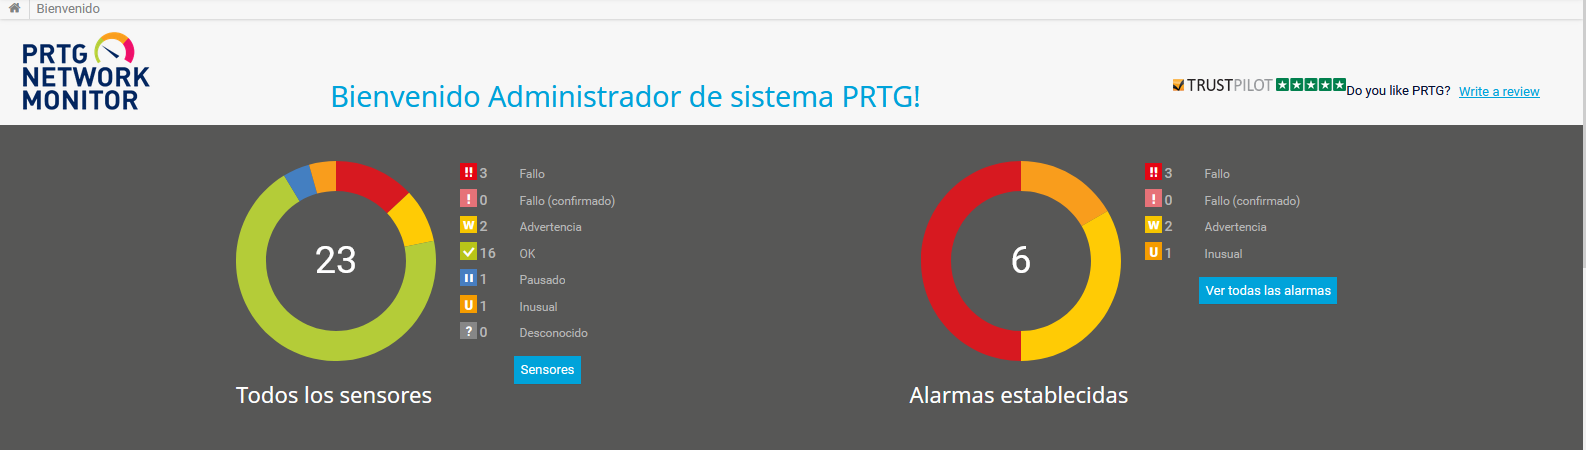
\includegraphics[width=1.1\textwidth]{img/img_prtg_inicio.png}
	\caption{inicio PRTG}
	\label{img_prtg_inicio}
\end{figure}

\begin{figure}[h]
	\centering
	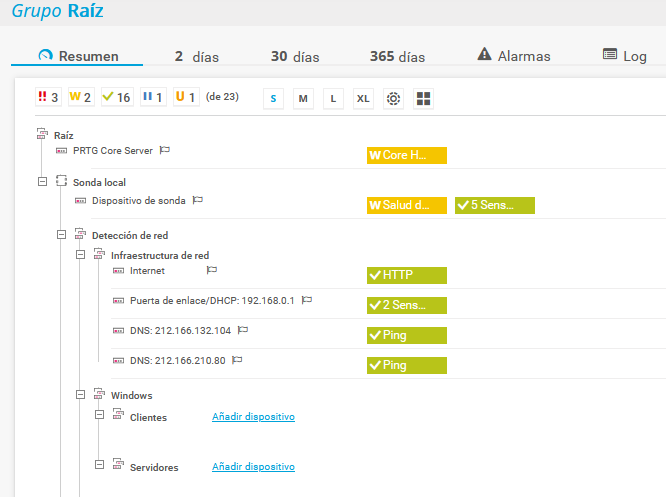
\includegraphics[width=1.1\textwidth]{img/img_prtg_dispositivos.png}
	\caption{dispositivos PRTG}
	\label{img_prtg_dispositivos}
\end{figure}

\begin{figure}[h]
	\centering
	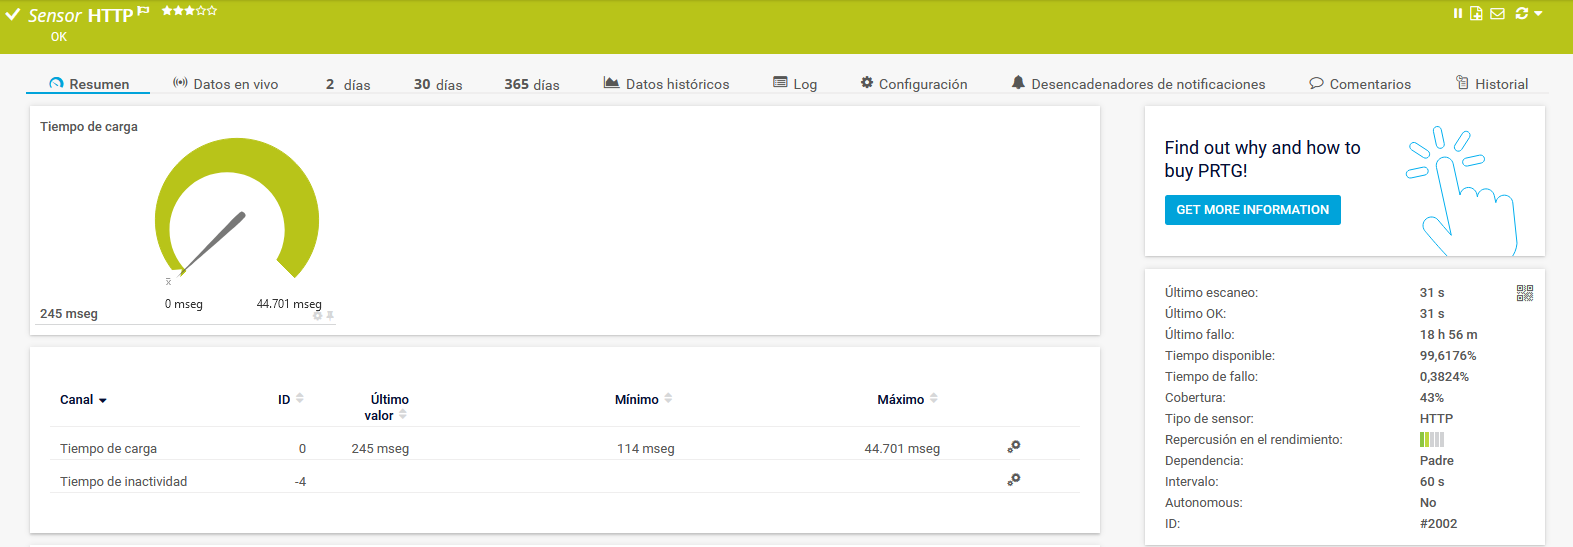
\includegraphics[width=1.1\textwidth]{img/img_ejemplo sensor.png}
	\caption{ejemplo sensor PRTG}
	\label{img_ejemplo}
\end{figure}

\clearpage

\section{Manual del usuario}

Este apartado pretende hacer de guía al usuario a través de la aplicación, mostrando cómo funciona el sistema y cómo es posible configurarlo.

\subsection{Configuración}

 Una vez se haya instalado \nombrePrograma hay una serie de modificaciones que hay que realizar manualmente antes de poder ser ejecutado.
 
\subsubsection{Logstash}

 El primero sería en el fichero del logstash, el cual se encuentra en la ruta: \textit{/etc/logstash/conf.d/logstashSensor.conf}
 
 En él se encuentra el mecanismo que permite a logstash procesar los archivos de logs con los datos de los sensores y enviárselos a la BBDD de Elasticsearch.
 
 \begin{verbatim}
input{
        http{
                id=> "sensor_data_http_input"
        }
}

filter{

        ruby {
                code => '
                    event.get("reading").each { |k, v|
                        event.set(k,v)
                    }
                    event.remove("reading")
                '
            }

}
output{

        elasticsearch{
                hosts => ["localhost:9200", "IP_Ubuntu_server:9200"]
                index => "sensor_data-%{+YYYY.MM.dd}"
        }
}
 \end{verbatim}
 
Para que logstash mande la información a Elasticsearch hay que sustituir donde pone ``IP\_Ubuntu\_server'' por la IP de Ubuntu server, en el cual se ha instalado Elasticsearch.

\subsubsection{Índice}

Logstash ahora ya sabe a dónde enviar los datos, pero se ha de preparar Elasticsearch para su llegada, se ha de crear un índice que diga a Elasticsearch que datos esperar.

Para ello se ha de acceder a la página principal de Elastic, introduciendo en un navegador web del host la url: \textit{IP\_Ubuntu\_server:5601}, donde \textit{IP\_Ubuntu\_server} es la ip del servidor.

Una vez se haya accedido a Elastic, para crear un índice se ha de acceder a \textit{Dev Tools}, accediendo desde el menú desplegable izquierdo, en el apartado de \textit{Management} se ha de introducir el POST con el índice \ref{indice} y enviar la \textit{request} cómo se puede observar en la figura \ref{img_index}



\begin{listing}
\begin{minted}[frame=single,
               framesep=3mm,
               linenos=true,
               xleftmargin=21pt,
               tabsize=6]{js}

POST _template/sensor_data_template
{
  "index_patterns": [
    "sensor_data*"
  ],
  "settings": {
    "number_of_replicas": "1",
    "number_of_shards": "5"
  },
  "mappings": {
    "properties": {
      "sensorId": {
        "type": "integer"
      },
      "datetime":{
        "type": "date",
        "format": "dd/MM/yyyy HH:mm:ss"
      },
      "reading": {
        "type": "nested", 
        "properties": { 
          "name": {"type":"keyword"},
          "description": {"type":"double"}
        }
      }
    }
  }
}


\end{minted}
\caption{Índice} 
\label{indice}
\end{listing}

\begin{figure}[h]
	\centering
	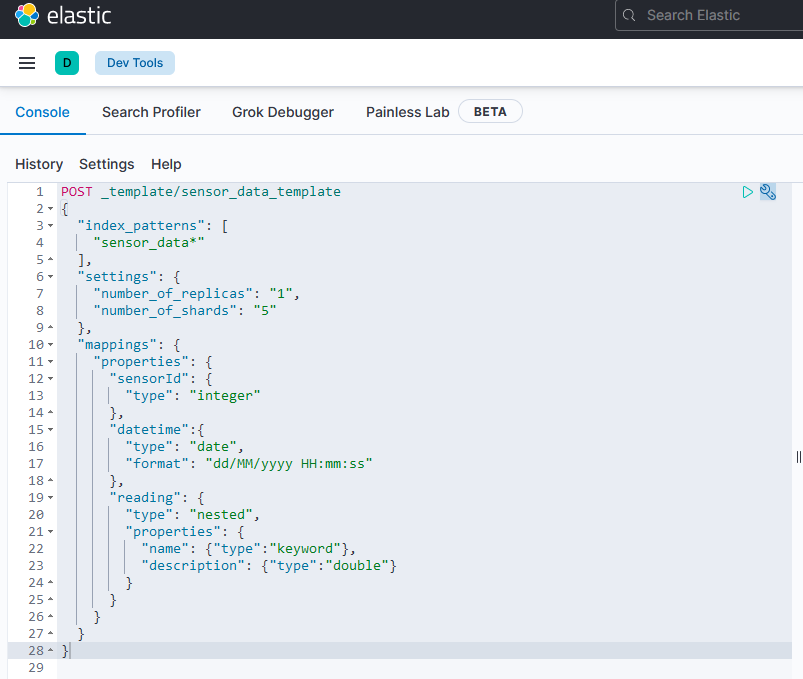
\includegraphics[width=1.1\textwidth]{img/img_crear_patron.png}
	\caption{Crear un índice}
	\label{img_index}
\end{figure}
\newpage

Una vez creado el índice todos los datos procedentes de losgstash se almacenarán con ese índice.
Dentro del menú \textit{Stack Management} en el apartado \textit{index Managment} se puede consultar los datos que va recibiendo \ref{img_index_manager.png}.

\begin{figure}[h]
	\centering
	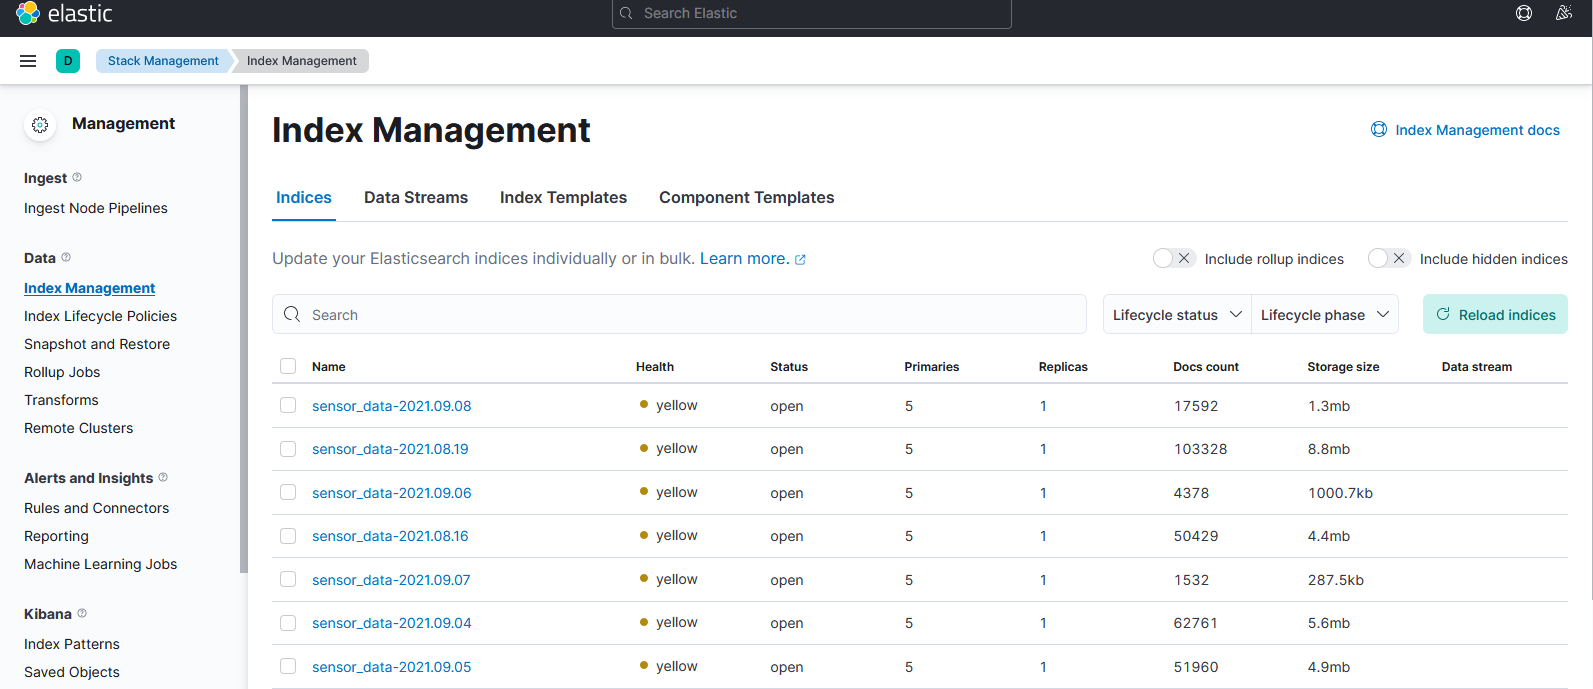
\includegraphics[width=1.1\textwidth]{img/img_index_manager.png}
	\caption{Index Managment}
	\label{img_index_manager.png}
\end{figure}

\newpage

\subsection{configuración de parámetros}

El usuario puede elegir que sensores desea almacenar y entrenar así cómo cada cuanto tiempo se desea ejecutar el programa y seleccionar cuantos instantes de tiempo en el futuro se desea predecir. Para ello se ha de acceder al fichero \textit{/usr/bin/Monitorizacion\_IOT/Monitorizacion\_IOT.sh} en él, se encintarán una serie de variables que el usuario ha de modificar.

\begin{itemize}
    \item \textbf{usuario\_PRTG}: se ha de introducir el nombre de usuario de PRTG
    \item \textbf{passhash\_PRTG}: se ha de introducir el passhash de PRTG
    \item \textbf{lista\_id\_sensor}: en esta lista se ha de introducir el id de los sensores, separados por un espacio.
    \item \textbf{horizonte\_predicción}: se ha de introducir cuantos minutos a futuro se desea que llegue la predicción.
    \item \textbf{repeticion\_ciclo}: Se ha de introducir el tiempo en segundos que ha de esperar el sistema entre ciclo y ciclo. 
\end{itemize}

Para saber la dirección IP de PRTG hay que acceder, dentro de PRTG a configuración > interfaz de usuario > combinaciones de puertos / servidor web direcciones IP activas y para saber el passhash se ha de acceder a configuración > mi cuenta > Configuración de cuenta de usuario y mostrar passhash.

\subsection{Crear un modelo para los sensores}

Para la realización del entrenamiento sobre los datos procedentes de un sensor, es esencial crear y configurar cada modelo a mano, respondiendo a las necesidades de estos.

Para crear un modelo hay que modificar de forma manual el fichero \textit{/usr/bin/Monitorizacion-IOT/Prediccion/Crear\_modelo.py}, una vez en el fichero, se ha de generar una instancia del modelo que se dese crear pasando cómo parámetro el id del sensor. A continuación, llamaremos a la función inicializar del modelo, pasándole los parámetros necesarios. Por último se llama al método guardar de la clase \textit{Persistencia\_modelo}. Para guardar el modelo simplemente compilamos el fichero, este se guardará en la carpeta \textit{/usr/bin/Monitorizacion-IOT/Prediccion/modelos/} y se podrá usar para el entrenamiento y la predicción.

\begin{verbatim}
if __name__ == "__main__":

    idSensor = 4051

    modelo = Modelo_SNARIMAX(idSensor)
    modelo.inicializar(q=2,
                        m=30,
                        sp=6,
                        sq=10,
                        intercept_init=12,
                        sgd=0.01, 
                        intercerpt_lr=0.3)

    Persistencia_modelo.guardar(modelo)

\end{verbatim}

\subsection{Inicialización y parada del sistema}

Una vez configurado el programa se puede inicializar y poner en marcha todo el sistema, para ello se ha de introducir el siguiente comando:

\begin{lstlisting}[frame=single]  
systemctl start Monitorizacion_IOT
\end{lstlisting}

para realizar la parada completa del sistema y que este deje de captar datos de PRTG se ha de introducir el siguiente comando:

\begin{lstlisting}[frame=single]  
systemctl stop Monitorizacion_IOT
\end{lstlisting}


\subsection{Index pattern}

Por último, para poder explorar y visualizar los datos en Kibana es necesarios que exista un ``index pattern'' que diga a Elasticsearch que índices contienen los datos, así como especificar de que tipo son. \cite{pagina:elastic}

Para poder crear un index pattern, primero Elasticsearch ha de tener datos \ref{img_index_pattern_antes_de_datos.png}, es por ello que este es el último paso a realizar.

Una vez se disponga de datos se podrá crear un index pattern \ref{img_index_patter_menu.png}

En este caso se ha de crear un patrón para que albergue todos los datos procedentes de sensores ``sensor\_data-*'' \ref{img_create_index_pattern.png}

\begin{figure}[h]
	\centering
	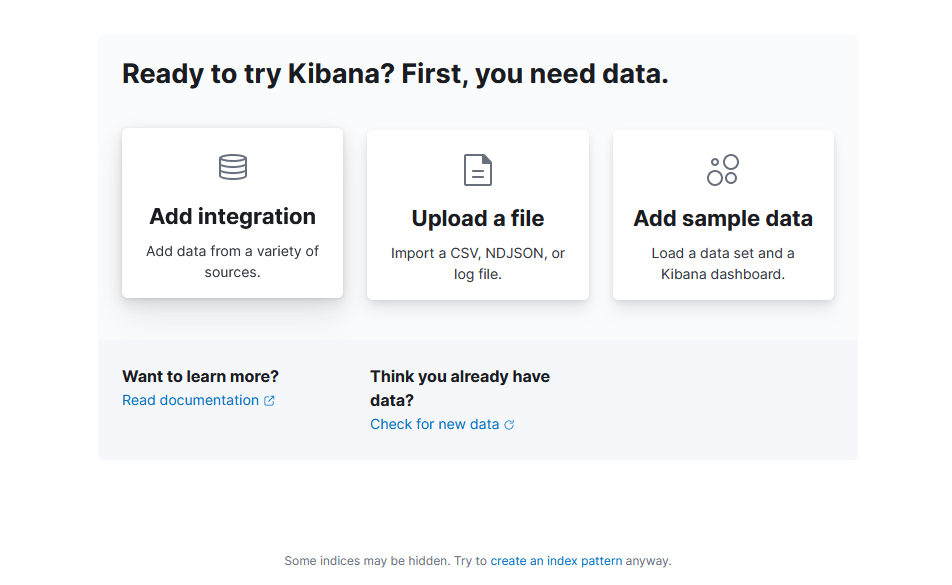
\includegraphics[width=1.1\textwidth]{img/img_index_pattern_antes_de_datos.png}
	\caption{Index pattern menú inicial si no se encuentran datos en Elasticsearch}
	\label{img_index_pattern_antes_de_datos.png}
\end{figure}

\begin{figure}[h]
	\centering
	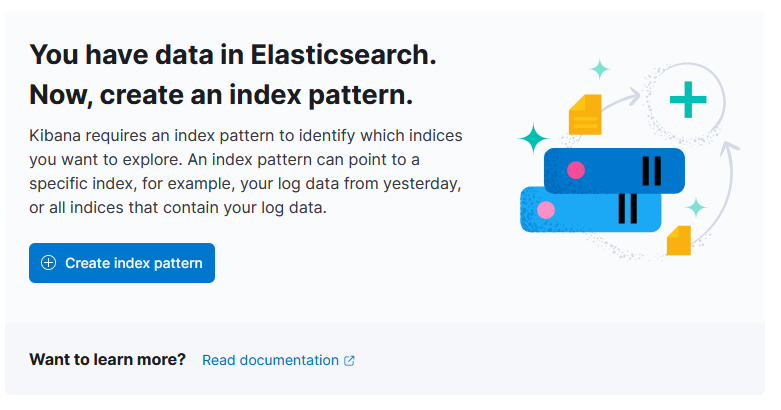
\includegraphics[width=1.1\textwidth]{img/img_index_patter_menu.png}
	\caption{Index pattern menú inicial}
	\label{img_index_patter_menu.png}
\end{figure}

\begin{figure}[h]
	\centering
	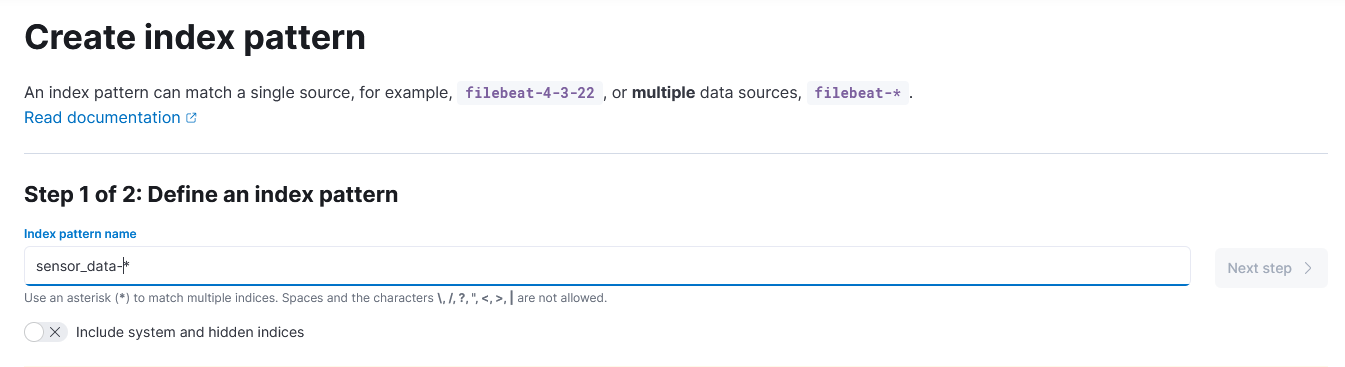
\includegraphics[width=1.1\textwidth]{img/img_create_index_pattern.png}
	\caption{Creación de un index pattern}
	\label{img_create_index_pattern.png}
\end{figure}

Una vez creado el patrón se pedirá que se configure, se puede especificar cuál va a ser el índice de los datos, si el tiempo en el que es indexado a en Elasticsearch ``@timestamp'' u otro campo fecha que se prefiera. \ref{img_conf_index_pattern.png}

También se puede cambiar el tipo de cualquier otro campo. 

\begin{figure}[h]
	\centering
	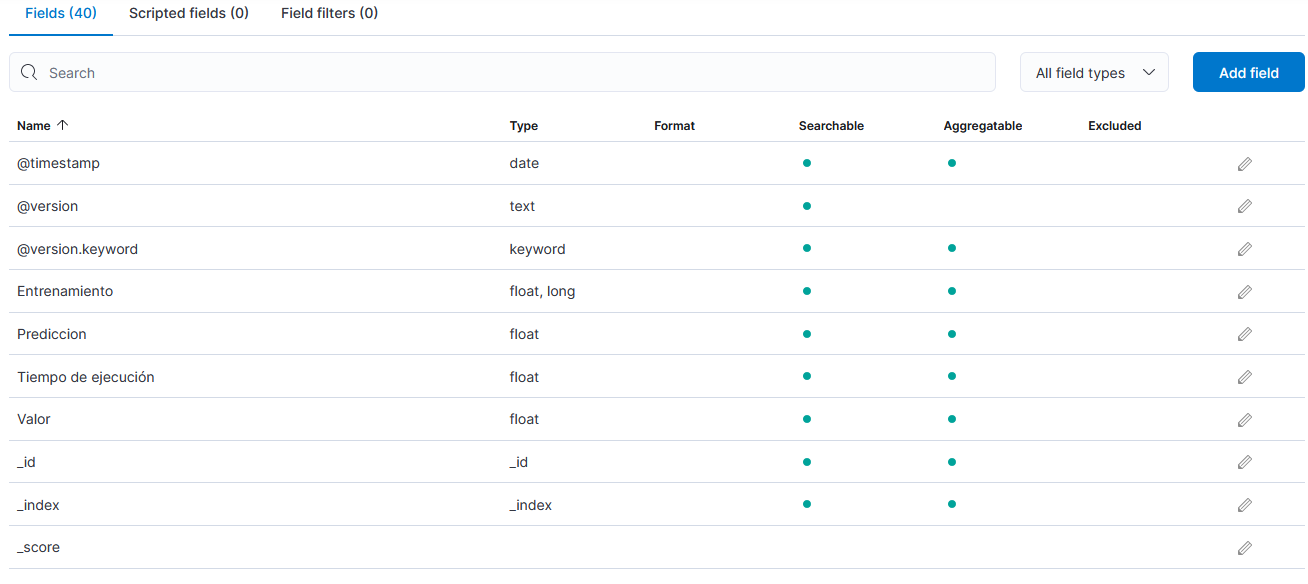
\includegraphics[width=1.1\textwidth]{img/img_conf_index_pattern.png}
	\caption{Configuración de un index pattern}
	\label{img_conf_index_pattern.png}
\end{figure}

\clearpage

\subsection{¿Cómo funciona \nombrePrograma?}

Una vez configurado e inicializado, el programa captará los datos de los sensores, los entrenará y realizará las predicciones. A continuación, se explicarán que proceses sigue. 

\nombrePrograma es un programa que se repite en bucle, cada ciclo se repite cada x tiempo, dependiendo del valor de la variable \textit{repeticion\_ciclo}. En cada ciclo se descargan, se entrenan y se predicen los datos de cada sensor. 

\subsubsection{Obtención y almacenamiento de datos}\label{cap:obt_alm_datos}

Para poder trabajar con los datos de los sensores, provenientes de PRTG es necesario descargarlos y almacenarlos para poder realizar el estudio y entrenamiento de dichos datos.

\nombrePrograma, mediante un script, descarga los datos de los sensores que se encuentran en la lista \textbf{lista\_id\_sensor}, estos se guardan en un fichero JSON, el cual se ha de transformar para adecuar el formato y que Elasticsearch pueda procesarlo. Para almacenar los datos ya obtenidos y transformados a la base de datos de Elasticsearch, estos ficheros son preprocesados por logstash que se encarga de enviar las líneas de datos al servidor de Elastic e indexarlos correctamente.

Los datos son subidos con el siguiente nombre: ``sensor\_data-yyyy.mm.dd'' de tal forma que todos los datos que se suben en un día se almacenan bajo un mismo índice. Para poder explorar y visualizar los datos en Kibana es necesarios que exista un ``index pattern'' que diga a Elasticsearch que índices contienen los datos, así como especificar de que tipo son, en este caso se ha creado uno para que albergue todos los datos procedentes de sensores ``sensor\_data-*''. 

Una vez los datos estén correctamente almacenados e indexados en Elasticsearch, se puede explorar y visualizar los datos con Kibana.


\newpage
\subsubsection{Transformación de datos}\label{cap:TransformacionDatos}

Durante la transformación de los ficheros JSON se eliminan los datos irrelevantes que se obtenían de PRTG, se añade el id del sensor y se cambia el formato de la fecha de dd/MM/yyyy H:mm:ss a dd/MM/yyyy HH:mm:ss.

Logstash esta preparado para trabajar con logs, es por eso que además también se separa cada entrada de datos por líneas, cómo se puede observar el los Listings \ref{json-example} y \ref{json-transformado-example}

\begin{listing}
\begin{minted}[frame=single,
               framesep=3mm,
               linenos=true,
               xleftmargin=21pt,
               tabsize=6]{js}
{
    "prtg-version":"21.2.68.1492",
    "treesize":30,
    "histdata":
    [
        {
            "datetime":"27/07/2021 16:11:06",
            "Valor":4.6800,
            "Tiempo de ejecución":782.0000,
            "coverage":"100 %"
        },
        {
            "datetime":"27/07/2021 16:12:06",
            "Valor":4.6800,
            "Tiempo de ejecución":797.0000,
            "coverage":"100 %"
        },
        {
            "datetime":"27/07/2021 16:13:06",
            "Valor":4.6700,
            "Tiempo de ejecución":799.0000,
            "coverage":"100 %"
        }
    ]
}

\end{minted}
\caption{JSON descargado de PRTG} 
\label{json-example}
\end{listing}

\begin{listing}
\begin{minted}[frame=single,
               framesep=3mm,
               linenos=true,
               xleftmargin=21pt,
               tabsize=6]{js}

{
    "sensorId":"2051",
    "datetime":"27/07/2021 16:11:06",
    "reading": 
    {
        "Valor":4.6800,
        "Tiempo de ejecución":782.0000
    }
}
{
    "sensorId":"2051",
    "datetime":"27/07/2021 16:12:06",
    "reading": 
    {
        "Valor":4.6800,
        "Tiempo de ejecución":797.0000
    }
}
{
    "sensorId":"2051",
    "datetime":"27/07/2021 16:13:06",
    "reading": 
    {
        "Valor":4.6700,
        "Tiempo de ejecución":799.0000
    }
}

\end{minted}
\caption{JSON transformado} 
\label{json-transformado-example}
\end{listing}

\newpage



\subsubsection{Machine learning}

\textbf{Incremental/Online Learning}

Cómo se ha especificado en el apartado de conceptos teóricos el incremental learning va entrenando el modelo con datos en un flujo continuo. Esto es muy beneficioso ya que en este proyecto en concreto no se dispone de muestras lo suficientemente grandes como para entrenar un modelo mediante la forma tradicional de \textit{batch learning} de forma eficaz. 

\textbf{Entrenamiento}

Una vez los datos de los sensores están correctamente indexados y almacenados en Elasticsearch se puede proceder al entrenamiento.

Por cada sensor se cargará el modelo que se haya creado para ese modelo en concreto y se descargarán los datos en un rango de fecha determinado desde Elasticsearch. Los valores de entrenamiento serán volcados a un fichero y devueltos a Elasticsearch, para poder monitorizar el entrenamiento.

Una vez se ha finalizado se guarda el modelo en disco para que la siguiente vez que se requiera entrenar modelo o hacer predicciones se utilice siempre el modelo más actualizado.

\textbf{Predicción}

Cada ciclo del programa se hace una predicción de los siguientes minutos (según se indique en la variable \textit{horizonte\_prediccion}), para no acumular datos repetidos en la BBDD, se eliminan los datos que se han predicho en el ciclo anterior. Así cada predicción que hace el programa esta actualizada.

Esta predicción se sube a Elasticsearch para poder ser visualizada.

\begin{figure}[h]
	\centering
	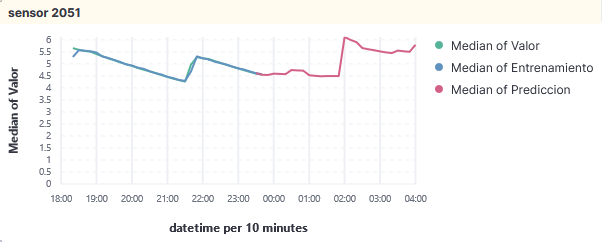
\includegraphics[width=1.1\textwidth]{img/img_prediccion_sensor2051.png}
	\caption{predicción sensor de Presión Tubería de Agua}
	\label{img_prediccion_sensor2051}
\end{figure}
\newpage


\subsection{Visualización y monitorización}

Mediante un navegador introducimos la siguiente url: IP\_ubuntu\_server:5601 (el puerto 5601 corresponde al de kibana).

\begin{figure}[h]
	\centering
	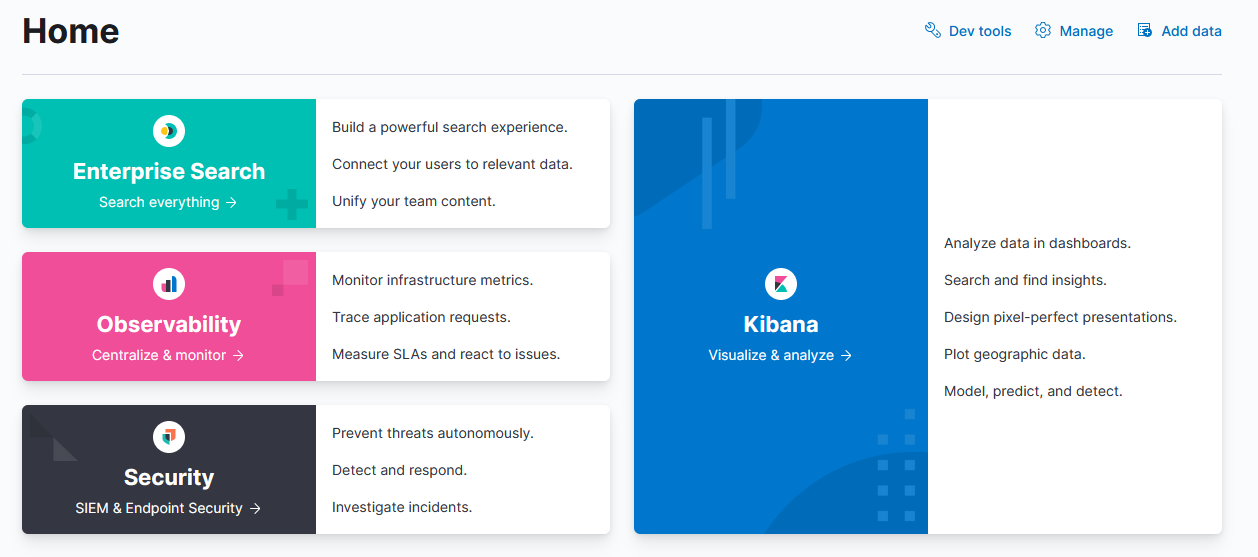
\includegraphics[width=1.1\textwidth]{img/img_kibana_home.png}
	\caption{pagina inicio kibana}
	\label{img_kibana_home}
\end{figure}

Una vez en el apartado home podemos acceder al apartado ``kibana Visualize \& analyze'' para poder echar un vistazo a nuestros datos. Para ver nuestros datos, así como realizar filtrados y búsquedas accederemos a ``Discover''

Se pueden visualizar los datos que estén vinculados a un patrón de índices.

\begin{figure}[h]
	\centering
	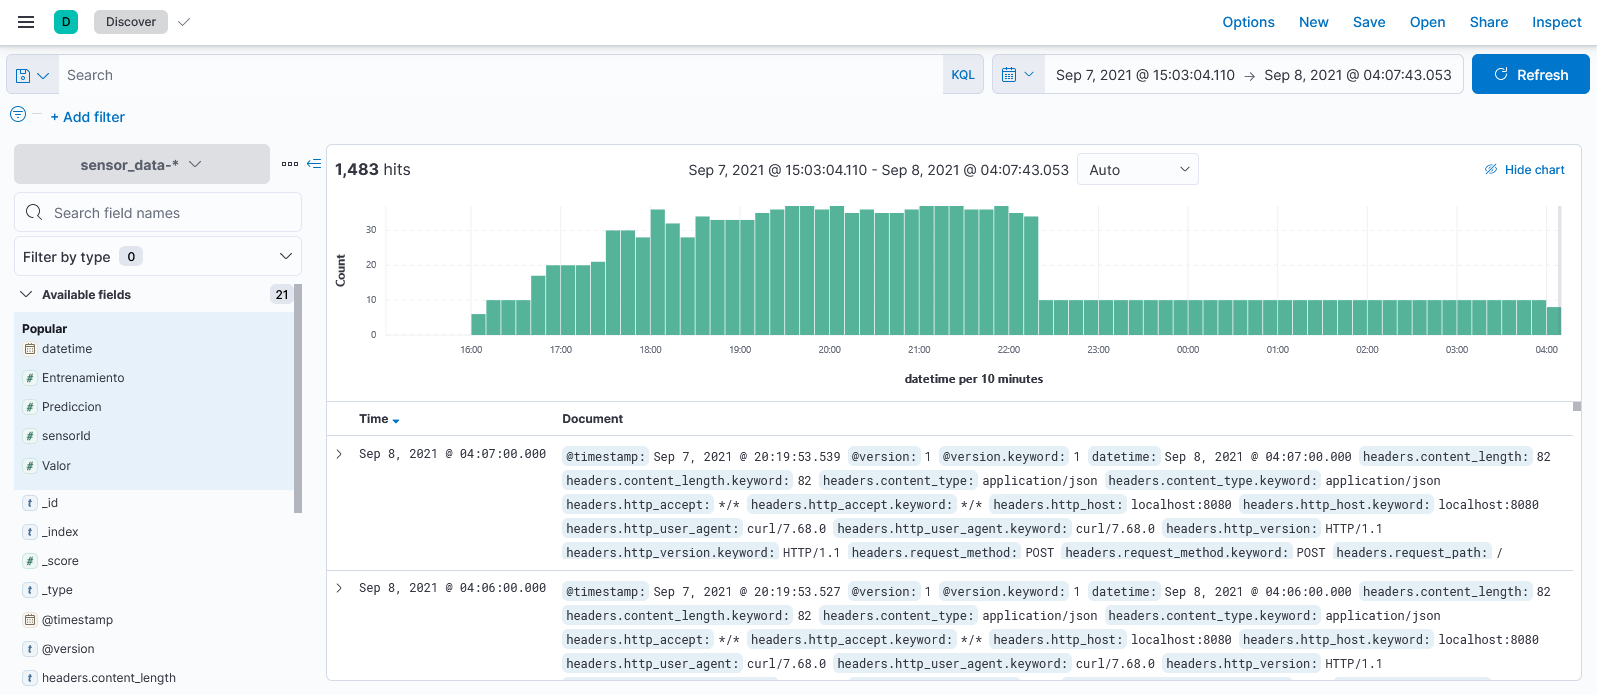
\includegraphics[width=1.1\textwidth]{img/img_kibana_discover.png}
	\caption{kibana discover}
	\label{img_kibana_discover}
\end{figure}

Para visualizar de forma gráfica los datos se ha de acceder al apartado ``Dashboard'' en él se puede crear cualquier tipo de gráfico.

\begin{figure}[h]
	\centering
	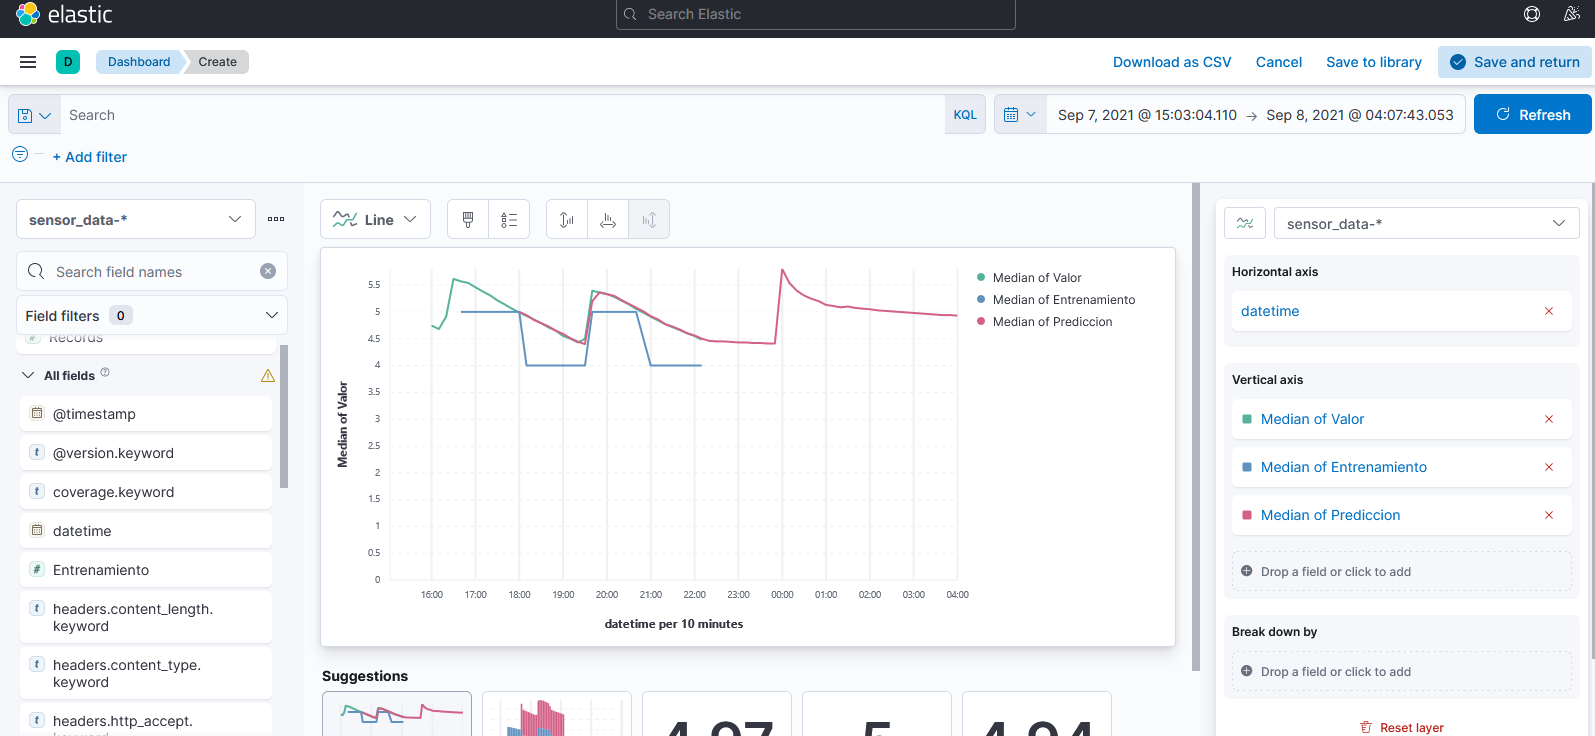
\includegraphics[width=1.1\textwidth]{img/img_kibana_dashboard.png}
	\caption{kibana dashboard}
	\label{img_kibana_dashboard}
\end{figure}


\subsection{Búsquedas y filtrados de datos}

kibana provee varias formas de construir queries con las cuales poder hacer filtrados y búsquedas en los datos almacenados en Elasticsearch.

En el apartado \textit{Discover} se muestran los datos de un índice, se pueden realizar una serie de filtrados y búsquedas, el filtrado de tiempo limita los datos mostrados en un rango de fechas, este filtrado, normalmente, se aplica al campo de tiempo del \textit{intex pattern}

\begin{figure}[h]
	\centering
	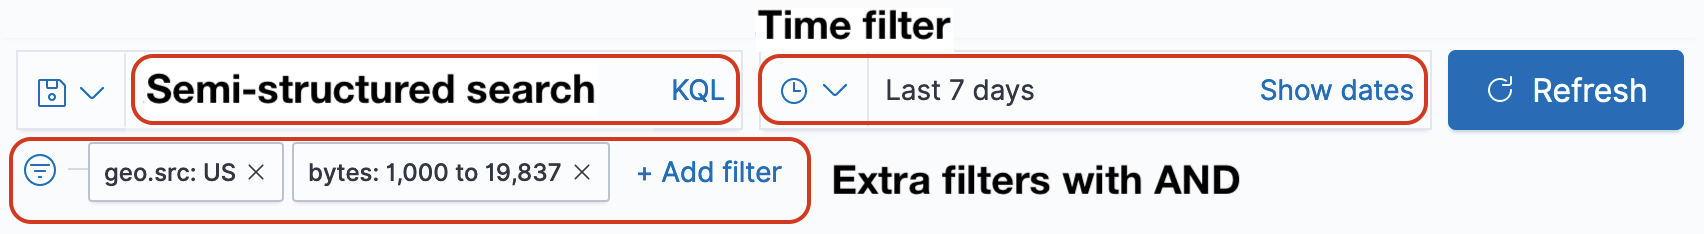
\includegraphics[width=1.1\textwidth]{img/img_time_filter.png}
	\caption{kibana filtrados}
	\label{img_time_filter.png}
\end{figure}

La sintaxis que se utilizada es KQL (Kibana Query Language) un lenguaje creado específicamente para facilitar las búsquedas y filtrados en Elasticsearch. \cite{pagina:KQL}

\begin{figure}[h]
	\centering
	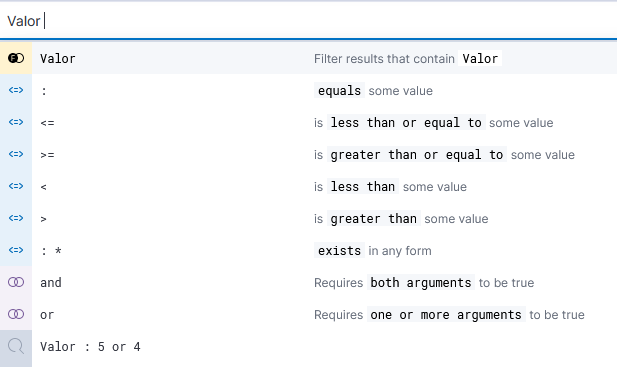
\includegraphics[width=1.1\textwidth]{img/img_fitradoDatos.png}
	\caption{kibana ayuda de filtrado}
	\label{img_fitradoDatos.png}
\end{figure}



\bibliographystyle{plain}
\bibliography{bibliografiaAnexos}

\end{document}
